%%%%%%%%%%%%%%%%%%%%%%%%%%%%%%%%%%%%%%%%%%%%%%%%%%%%%%%%%%%%%%%%%%%%%%%%%%%%%%%%
%%% USE 80 character line lengths with linebreaks (Emacs-style)
%%%%%%%%%%%%%%%%%%%%%%%%%%%%%%%%%%%%%%%%%%%%%%%%%%%%%%%%%%%%%%%%%%%%%%%%%%%%%%%%

\documentclass[reprint,onecolumn,superscriptaddress]{revtex4-1}

\usepackage{amsmath}
\usepackage{amssymb}
\usepackage{graphicx}
\usepackage[version=3]{mhchem}
\usepackage{physics}
\usepackage{xfrac}
\usepackage{gensymb}
\usepackage{xcolor}
\usepackage[utf8]{inputenc}

\usepackage[hidelinks]{hyperref}

\graphicspath{{./figures/}}

\newcommand{\dftbp}{DFTB+}

\begin{document}

\title{\dftbp{}, a software package for efficient approximate density functional
  theory based atomistic simulations}

\author{B. Hourahine} \affiliation{SUPA, Department of Physics, The University
  of Strathclyde, Glasgow, G4 0NG, United Kingdom}

\author{B. Aradi}
%\email[corresponding author, e-mail:~]{aradi@uni-bremen.de}
\affiliation{Bremen Center for Computational Materials Science, University of
  Bremen, Bremen, Germany}

\author{V. Blum}
\affiliation{Department of Mechanical Engineering and Materials Science, Duke
  University, Durham, NC, USA}

\author{F. Bonaf\'e}
\affiliation{Max Planck Institute for the Structure and
  Dynamics of Matter, Hamburg, Germany}

\author{A. Buccheri} \affiliation{School of Chemistry, University of Bristol,
  Cantock's Close, Bristol, BS8 1TS, United Kingdom}

\author{C. Camacho}
\affiliation{School of Chemistry, University of Costa Rica, San Jos\'e,
  11501-2060, Costa Rica}

\author{C. Cevallos}
\affiliation{School of Chemistry, University of Costa Rica, San Jos\'e,
  11501-2060, Costa Rica}

\author{M. Y. Deshaye}
\affiliation{Department of Chemistry and Advanced Materials Science \&
  Engineering Center, Western Washington University, Bellingham, WA, USA}

\author{T. Dumitric\u{a}}
\affiliation{Department of Mechanical Engineering, University of Minnesota,
  Minneapolis, USA}

\author{A. Dominguez}
\affiliation{Bremen Center for Computational Materials Science, University of
  Bremen, Bremen, Germany}
\affiliation{Computational Science Research Center (CSRC) Beijing and Computational Science Applied Research (CSAR) Institute Shenzhen, China}

\author{S. Ehlert}
\affiliation{University of Bonn, Bonn, Germany}

\author{M. Elstner}
\affiliation{Institute of Physical Chemistry, Karlsruhe Institute of Technology,
  Karlsruhe, Germany}

\author{T. van der Heide}
\affiliation{Bremen Center for Computational Materials Science, University of
  Bremen, Bremen, Germany}

\author{J. Hermann}
\affiliation{Freie Universit\"at Berlin, Berlin, Germany}

\author{S. Irle}
\affiliation{Oak Ridge National Laboratory, USA}

\author{J. J. Kranz}
\affiliation{Institute of Physical Chemistry, Karlsruhe Institute of Technology,
  Karlsruhe, Germany}

\author{C. K{\"o}hler}
\affiliation{Bremen Center for Computational Materials Science, University of
  Bremen, Bremen, Germany}

\author{T. Kowalczyk}
\affiliation{Department of Chemistry and Advanced Materials Science \&
  Engineering Center, Western Washington University, Bellingham, WA, USA}

\author{T. Kuba\v{r}}
\affiliation{Institute of Physical Chemistry, Karlsruhe Institute of Technology,
  Karlsruhe, Germany}

\author{I. S. Lee}
\affiliation{Department
  of Chemistry, Ulsan National Institute of Science and Technology, South Korea}

\author{V. Lutsker}
\affiliation{Institut I -- Theoretische Physik, University of Regensburg,
  Regensburg, Germany}

\author{R. J. Maurer}
\affiliation{Department of Chemistry, University of Warwick, Gibbet Hill Road,
  Coventry, CV4 7AL, UK}

\author{S. K. Min}
\affiliation{Department
  of Chemistry, Ulsan National Institute of Science and Technology, South Korea}

\author{I. Mitchell}
\affiliation{Center for Multidimensional Carbon Materials, Institute of Basic
  Science, South Korea}

\author{C. Negre}
\affiliation{Theoretical Division, Los Alamos National Laboratory, USA}

\author{T. A. Niehaus}
\affiliation{Univ Lyon, Universit\'e Claude Bernard Lyon 1, CNRS,
  Institut Lumi\`ere Mati\`ere, F-69622, Villeurbanne, France.}

\author{A. M. N. Niklasson}
\affiliation{Theoretical Division, Los Alamos National Laboratory, USA}

\author{A. J. Page}
\affiliation{School of Environmental and Life Sciences, University of Newcastle, Australia}

\author{A. Pecchia}
\affiliation{CNR-ISMN, Via Salaria km 29,600, 00014 Monterotondo, Rome}

\author{G. Penazzi}
\affiliation{Bremen Center for Computational Materials Science, University of
  Bremen, Bremen, Germany}

\author{M. P. Persson}
\affiliation{Dassault Systemes, Cambridge, United Kingdom}

\author{J. \v{R}ez\'a\v{c}}
\affiliation{Institute of Organic Chemistry and Biochemistry AS CR, Prague, Czech Republic}

\author{C. G. S\'anchez}
\affiliation{Instituto Interdisciplinario de Ciencias B\'asicas, Universidad
  Nacional de Cuyo, CONICET, Facultad de Ciencias Exactas y Naturales, Mendoza,
  Argentina}

\author{M. Sternberg}
\affiliation{Argonne National Laboratory, USA}

\author{M. St\"ohr}
\affiliation{Department of Physics and Materials Science, University of
  Luxembourg, Luxembourg}

\author{F. Stuckenberg}
\affiliation{Bremen Center for Computational Materials Science, University of
  Bremen, Bremen, Germany}

\author{A. Tkatchenko}
\affiliation{Department of Physics and Materials Science, University of
  Luxembourg, Luxembourg}

\author{V. W.-z.~Yu}
\affiliation{Department of Mechanical Engineering and Materials Science, Duke
  University, Durham, NC, USA}

\author{T. Frauenheim}
\affiliation{Bremen Center for Computational Materials Science, University of
  Bremen, Bremen, Germany}
\affiliation{Computational Science Research Center (CSRC) Beijing and Computational Science Applied Research (CSAR) Institute Shenzhen, China}


\date{\today}

\begin{abstract}
  \dftbp{} is a versatile community developed open source software package
  offering fast and efficient methods for carrying out atomistic quantum
  mechanical simulations. By implementing various methods approximating density
  functional theory (DFT), like the density functional based tight binding
  (DFTB) and the extended tight binding (xTB) method, it enables simulations of
  large systems and long timescales with reasonable accuracy while being
  considerably faster for typical simulations than respective \textit{ab initio}
  methods. Based on the DFTB framework it additionally offers approximated
  versions of various DFT extensions including hybrid functionals, time
  dependent formalism for treating excited systems, electron transport using
  non-equilibrium Green's functions and many more. \dftbp{} can be used as a
  user-friendly standalone application as well as being embedded into other
  software packages as a library or acting as a calculation-server accessed by
  socket communication. We give an overview of the recently developed
  capabilities of the \dftbp{} code, demonstrating with a few use case examples,
  discuss the strengths and weaknesses of the various features and discuss
  on-going developments and possible future perspectives.

  \bigskip

  \noindent
  This $\Psi_k$ Scientific Highlight has been adapted from
  \href{https://doi.org/10.1063/1.5143190}{\color{blue}{J. Chem.\ Phys.\ 152, 124101 (2020)}}
  with the permission of AIP Publishing and is licenced under
  \href{http://creativecommons.org/licenses/by/4.0/}{\color{blue}{CC BY 4.0}}.

\end{abstract}


\maketitle

\section{Introduction}

Density Functional Theory (DFT)~\cite{Hohenberg1964,Kohn1965} dominates the
landscape of electronic structure methods, being the usual go-to technique to
model large, chemically complex systems at good accuracy. For larger systems and
time scales, force-field models instead dominate materials and chemical
modeling. Between these is the domain of semi-empirical methods, derived from
approximations to Hartree-Fock or DFT based methods. Within this space, density
functional based tight binding
(DFTB)~\cite{Seifert1996,Porezag1995,Elstner1998}, effectively offers a reduced
complexity DFT method, being derived from a simplification of Kohn-Sham DFT to a
tight binding form~\cite{ElstnerSeifertBBA2014}.

This article describes the \dftbp{} code~\cite{dftbplus-repo}, an open source
implementation which aims to collect the developments of this family of methods
and make them generally available to the chemical, materials and condensed
matter communities. This article describes extensions to this code since its
original release in 2007 \cite{aradi-jpca-2007}.

\section{\dftbp{} features}

\subsection{The core DFTB-model}

The basic DFTB-equations are presented below. They can be easily generalized for
periodic cases ($k$-points) as well as for other boundary conditions, as
implemented in \dftbp{}. All equations throughout are given in atomic units with
Hartree as the energy unit.

\subsubsection{Expansion of the total energy}

The DFTB models are derived from Kohn-Sham (KS) DFT~\cite{Kohn1965}
by expansion of the total energy functional.  Starting from a properly
chosen reference density $\rho_0$ (e.g.\ superposition of neutral atomic
densities), the ground state density is then represented by this reference, as 
perturbed by density fluctuations:
$\rho(\mathbf{r}) = \rho_0(\mathbf{r}) +\delta\rho(\mathbf{r})$.  The total
energy expression then expands the energy functional in a Taylor series up to third
order:
\begin{equation}
  E^{\text{DFTB3}}[\rho_0+\delta\rho] = E^0[\rho_0] + E^1[\rho_0,\delta \rho] +
  E^2[\rho_0,(\delta \rho)^2] + E^3[\rho_0,(\delta \rho)^3]
\end{equation}
with
\begin{eqnarray}
  E^0[\rho_0] &=& \frac 12 \sum_{AB} \frac{Z_AZ_B}{R_{AB}} -\frac 12 \iint
  \frac{\rho_0(\mathbf{r})\rho_0(\mathbf{r}')}{|\mathbf{r}-\mathbf{r}'|}
  \mathrm{d}\mathbf{r} \mathrm{d}\mathbf{r}' -\int
  V^{\text{xc}}[\rho_0]\rho_0(\mathbf{r})\text{d}\mathbf{r} +
  E^{\text{xc}}[\rho_0] \nonumber\\ E^1[\rho_0,\delta \rho] &=& \sum_i n_i
  \mel{\psi_i}{\hat{H}[\rho_0]}{\psi_i} \nonumber\\ E^2[\rho_0,(\delta \rho)^2]
  &=& \frac{1}{2} \iint \left( \frac{1}{|\mathbf{r}-\mathbf{r}'|} + \eval{
    \frac{\delta^2E^{\text{xc}}[\rho]}{\delta\rho(\mathbf{r})
      \delta\rho(\mathbf{r}')} }_{\rho_0} \right) \delta\rho(\mathbf{r})
  \delta\rho(\mathbf{r}') \mathrm{d}\mathbf{r} \mathrm{d}\mathbf{r}' \nonumber
  \\ E^3[\rho_0,(\delta \rho)^3] &=& \frac{1}{6} \iiint \eval{
    \frac{\delta^3E^{\text{xc}}[\rho]}{\delta\rho(\mathbf{r})
      \delta\rho(\mathbf{r}') \delta\rho(\mathbf{r}'')} }_{\rho_0}
  \delta\rho(\mathbf{r}) \delta\rho(\mathbf{r}') \delta\rho(\mathbf{r}'')
  \mathrm{d}\mathbf{r} \mathrm{d}\mathbf{r}'
  \mathrm{d}\mathbf{r}'',\label{DFTtaylor}
\end{eqnarray}
with XC being the exchange correlation energy and potential.
%
Several DFTB models have been implemented, starting from the first order
non-self-consistent DFTB1~\cite{Seifert1996,Porezag1995} (originally called
DFTB or non-SCC DFTB), the second order DFTB2 (originally called SCC-DFTB)~\cite{Elstner1998}
and the more recent extension to third order,
DFTB3~\cite{Elstner2007,Yang2007,Gaus2011,Gaus2012}.

\subsubsection{DFTB1}

The first order DFTB1 method is based on three major approximations: (i) it
takes only $E^0[\rho_0]$ and $ E^1[\rho_0,\delta \rho]$ from
Eq.~\eqref{DFTtaylor} into account, (ii) is based on a valence-only minimal
basis set ($\phi_\mu$) within a linear combination of atomic orbitals (LCAO)
{\it ansatz}
\begin{equation}
  \psi_i=\sum_\mu c_{\mu i}\phi_\mu
\end{equation}
for the orbitals $\psi_i$ (iii) and applies a two-center approximation to the
hamiltonian operator $\hat{H}[\rho_0]$.

\paragraph{Minimal atomic basis set}
The atomic orbital basis set $\phi_\mu$ is explicitly computed from DFT by
solving the atomic Kohn-Sham equations with an additional (usually harmonic)
confining potential:
\begin{equation}
  \left[ -\frac{1}{2} \nabla^2 + V^{\mbox{\scriptsize
        eff}}[\rho^{\mbox{\scriptsize atom}}] + \left( \frac{r}{r_0}\right)^n
    \right] \phi_{\mu} = \epsilon_{\mu} \phi_{\mu} \text.\label{eqn:DFTBatom}
\end{equation}
This leads to slightly compressed atomic-like orbitals for describing the
density in bonding situations. The actual values for $r_0$ are usually given in
the publications describing the specific parameterization.  The operator
$\hat{H}[\rho^0]$ also depends on the superposition of atomic densities,
$\rho_A$ (or potentials, $V_A^\text{eff}$) of neutral atoms, $\{A\}$, in the
geometry being modeled.  This density is usually determined from the same atomic
KS equations, using a slightly different confinement radius, $r_0^\text{d}$.


\paragraph{DFTB matrix elements}

The hamiltonian can be represented in an LCAO basis as
\begin{eqnarray}
  H_{\mu\nu}^0 = \mel{\phi_{\mu}}{\hat{H}[\rho_0]}{\phi_{\nu}} \approx
  \mel{\phi_{\mu}}{- \frac{1}{2} \nabla^2 +V[\rho_A +
      \rho_B]}{\phi_{\nu}}\qquad{\mu \in A, \nu \in B},
  \label{eqn:matelements}
\end{eqnarray}
where the neglect of the three center terms and pseudo-potential
contributions~\cite{ElstnerSeifertBBA2014} lead to a representation which can be
easily computed by evaluating the Kohn-Sham equations for dimers. These matrix
elements are computed once as a function of inter-atomic distance for all element
pairs. The Slater-Koster~\cite{PhysRev.94.1498} combination rules are applied for
the actual orientation of these `dimers' within a molecule or solid.

\paragraph{Total energy}
$E^0[\rho_0]$ depends only on the reference density so is universal, in that
sense that is does not specifically depend on the chemical environment (which
would determine any charge transfer, $\delta \rho$, occurring). It can
therefore be determined for a ``reference system'' and then applied to other
environments. This is the key to transferability of the parameters. In DFTB,
$E^0[\rho_0]$ is approximated as a sum of pair potentials called repulsive
energy terms,
\begin{eqnarray}
  E^0[\rho_0] \approx E_\text{rep} = \frac{1}{2}\sum_{AB}V^{\text{rep}}_{AB},
  \label{eq:erep}
\end{eqnarray}
(see Ref.~\cite{Seifert2012}) which are either determined by comparison
with DFT calculations~\cite{Porezag1995} or fitted to empirical
data~\cite{Gaus2009}. Forces are calculated with the Hellmann-Feynman theorem and
derivatives of the repulsive energy.


\subsubsection{DFTB2 and DFTB3}
\label{sec:dftb2}
To approximate the $E^2$ and $E^3$ terms in Eq.~\eqref{DFTtaylor} the density
fluctuations are written as a superposition of atomic contributions,
taken to be exponentially decaying spherically symmetric charge densities
\begin{eqnarray}
  \delta\rho(\mathbf{r}) = \sum_A \delta \rho_A(\mathbf{r} - \mathbf{R}_A)
  \approx \frac{1}{\sqrt{4\pi}} \sum_A \left( \frac{\tau_A^3}{8\pi}
  \mathrm{e}^{-\tau_A|\mathbf{r}-\mathbf{R}_A|} \right) \Delta q_A \text.
\end{eqnarray}
By neglecting the XC-contributions for the moment, the second order integral
$E^2$ leads to an analytical function, $\gamma_{AB}$, with
energy~\cite{Elstner1998}:
%
\begin{eqnarray}
  E^2(\tau_A,\tau_B,R_{AB}) = \frac{1}{2}\sum_{AB(\ne A)}
  \gamma_{AB}(\tau_A,\tau_B,R_{AB}) \Delta q_A \Delta q_B.\label{spin2}
\end{eqnarray}
%
The energy depends on the Mulliken charges $\{q_A\}$ (where the atomic charge
fluctuation, $\Delta q_A = q_A - Z_A$, is with respect to the neutral atom)
which are in turn dependent on the molecular orbital coefficients, $c_{\mu
  i}$. Thus, the resulting equations have to be solved self-consistently. At
large distances $\gamma_{AB}$ approaches $1/R_{AB}$, while at short distances it
represents electron-electron interactions within one atom.  For the limit
$R_{AB}\rightarrow 0$ one finds $\tau_A = \frac{16}{5} U_A$, i.e., the so called
Hubbard parameter $U_A$ (twice the chemical hardness) is inversely proportional
to the width of the atomic charge density $\tau_A$. This relation is intuitive
in that more diffuse atoms (or anions) have a smaller chemical hardness. For
DFTB the chemical hardness is computed from DFT, not fitted.

The third order terms describe the change of the chemical hardness of an atom
and are also computed from DFT. A function $\Gamma_{AB}$ results as the
derivative of the $\gamma$-function with respect to charge, and the DFTB3 total
energy is then given by
\begin{equation}
  E^{\text{DFTB3}} = \sum_i \sum_{AB}\sum_{\mu\in A}\sum_{\nu\in B} n_i c_{\mu i}
  c_{\nu i} H^0_{\mu\nu} + \frac{1}{2}\sum_{AB} \Delta q_A \Delta
  q_B\gamma_{AB}^h
  + \frac{1}{3}\sum_{AB} \Delta q_A^2 \Delta q_B\Gamma_{AB} +
  \frac{1}{2}\sum_{AB}V^{\text{rep}}_{AB}.
  \label{eq:etot}
\end{equation}
%
The third order terms become important when local densities deviate
significantly from the reference, i.e.\ $\Delta q_A$ is large. Apart from
including the third order terms, DFTB3 also modifies $\gamma_{AB}$ for the
interactions between hydrogen and first row elements~\cite{Elstner2007}, where
the deviation from the relation between the charge width and the chemical
hardness, as formulated above, is most pronounced.

The resulting DFTB3 hamiltonian takes the form
\begin{align}
H_{\mu\nu} &= H^0_{\mu\nu} + H^2_{\mu\nu}[\gamma^h,\Delta q] + H^3_{\mu\nu}[\Gamma,\Delta q] \qquad{\mu \in A, \nu \in B} \label{dftb3Ham}\\
H^2_{\mu\nu} &= \frac{S_{\mu\nu}}{2} \sum\limits_C \left( \gamma^h_{BC} + \gamma^h_{AC} \right) \Delta q_C\\
H^3_{\mu\nu} &= S_{\mu\nu} \sum\limits_C \left( \frac{\Delta q_A \Gamma_{AC}}{3} + \frac{\Delta q_B
\Gamma_{BC}}{3} + \left( \Gamma_{AC} + \Gamma_{BC}
\right) \frac{\Delta q_c}{6} \right) \Delta q_C
\end{align}
where $S_{\mu\nu}$ is the overlap matrix between orbitals $\phi_\mu$ and
$\phi_\nu$, and $\gamma^h$ is the modified DFTB2 interaction.

\subsubsection{Spin}

Analogous to DFTB2, expanding the energy with respect to spin
fluctuations~\cite{Frauenheim2000, Koehler2005, Koehler2001} leads to the
spin-polarized expressions for DFTB. By introducing the magnetization density
$m(\mathbf{r})=\rho^{\uparrow}(\mathbf{r})-\rho^{\downarrow}(\mathbf{r})$ as
difference of the densities of spin-up and spin-down electrons and its
corresponding fluctuations ($\delta m(\mathbf{r})$) around the spin-unpolarized
reference state ($|m(\mathbf{r})|=0$), a spin dependent term is added to the
spin-independent $E^2$ of Eq.~\eqref{DFTtaylor}:
\begin{eqnarray}
E^2[\rho_0,(\delta \rho)^2,(\delta m)^2]
  &=& E^2[\rho_0,(\delta \rho)^2] 
  +\frac{1}{2}\int 
  \eval{\frac{\delta^2E^{\text{xc}}[\rho,m]}{\delta m(\mathbf{r})^2}}_{\rho_0,m=0}\delta m(\mathbf{r})^2\mathrm{d}\mathbf{r} \label{spin1}
\end{eqnarray}
where a local or semi-local $E^{\text{xc}}$ has been assumed.

Identifying the spin density fluctuations with up- and down-spin Mulliken charge
differences, $\Delta p_{Al}$, for angular momentum shell $l$ at atom $A$, and
approximating the second derivative of $E^{\text{xc}}[\rho,m]$ as an atomic
constant $W_{All'}$ (similar to the Hubbard $U_A$), leads to an on-site energy
contribution
\begin{equation}
  E^2_{spin}=\frac{1}{2}\sum_{A}\sum_{l \in A} \sum_{l' \in A} W_{All'} \Delta
  p_{Al}\Delta p_{Al'}.\label{spin3}
\end{equation}
This term in Eq.~\eqref{spin3} is to be added to Eq.~\eqref{spin2}. It captures
the spin-polarization contribution to the total energy and couples different
atomic angular momentum shells via a magnetic interaction. The $W_{All'}$ are
usually an order of magnitude less than the $U_A$ and are multiplied with a
(typically) small $\Delta p_{Al}$, hence inclusion of spin-polarization via
Eq.~\eqref{spin3} gives only a small energy contribution. If there is a net
imbalance of up- and down-spin electrons in the system, the occupation of
electronic states alone carries most of the effect of the unpaired electron(s)
without including Eq.~\eqref{spin3}.  The use of Mulliken charges leads to an
additional hamiltonian contribution~\cite{Koehler2005} to the (now) shell
resolved form of Eq.~\eqref{dftb3Ham},
\begin{equation}
  H^{spin\pm}_{\mu\nu} = \pm \frac{S_{\mu\nu}}{2} \left( \sum\limits_{l'' \in A}
  W_{All''}\Delta p_{Al''} + \sum\limits_{l'' \in B} W_{Bl'l''}\Delta
  p_{Bl''}\right)\qquad{\mu \in l \in A, \nu \in l' \in B,}\label{spin4}
\end{equation}
where the spin up (down) hamiltonian has this term added (subtracted).

Expanding further to local (not global) up and down spin populations via Pauli
spinors gives the non-collinear spin model~\cite{doi:10.1021/jp068802p}.
Eq.~\eqref{spin3} becomes
\begin{equation}
E^2_{spin} = \frac{1}{2}\sum_{A}\sum_{l \in A} \sum_{l' \in A} W_{All'} \Delta \vec{p}_{Al} \cdot \Delta \vec{p}_{Al'},\label{spin3nc}
\end{equation}
and the wave-function generalizes to two component spinors. The hamiltonian
contributions take the form
\begin{equation}
\left(H^0_{\mu\nu} + H^2_{\mu\nu} + H^3_{\mu\nu}\right) \otimes \mqty(\pmat{0}) + \sum_{i=1}^{3} H^{\sigma_i}_{\mu\nu} \otimes \sigma_i, 
\end{equation}
where $\sigma_i$ is the Pauli matrix for spin component $i (= x,y,z)$ and
$H^{\sigma_i}$ is constructed from the $i^\mathrm{th}$ spin component of $\Delta
\vec{p}$. This spin-block two component hamiltonian then also enables spin-orbit
coupling~\cite{doi:10.1021/jp068802p,Hourahine11} to be included in \dftbp{}. The
spin-block hamiltonian addition is
\begin{equation}
H_{\mu\nu}^{L \cdot S} = \frac{S_{\mu\nu}}{2} \otimes\left(  \xi_{Al} \mqty( L_z & L^-\\ L^+ & - L_z )_l + \xi_{Bl'} \mqty( L_z & L^-\\ L^+ & - L_z )_{l'} \right)\qquad{\mu \in l\in A, \nu \in l' \in B}
\end{equation}
where $\xi_{Al}$ is the spin orbit coupling constant for shell $l$ of atom $A$
with $L^\pm$ and $L_z$ the angular momentum operators for atomic shells.

\subsubsection{Limitations of the core DFTB-model}

DFTB is an approximate method, and as such shows limitations, which can be
traced back to the different approximations applied.  However, the fitting of
Eq.~\eqref{eq:erep} can compensate for some of the inaccuracies.  Since up to
now only bonding contributions are addressed by the two-center nature of the
repulsive potentials, bond-lengths, bond-stretch frequencies and bond-energies
can be targeted. Properties such as bond angles or dihedral angles can not be
influenced by repulsive pair parameterization.  This is the reason, why DFTB
performs better than a fixed minimal basis DFT method, which would be only of
limited use in most of the applications. In some cases DFTB can even perform
better than double-zeta (DZ) DFT using GGA functionals, as shown e.g.\ in
Ref.~\cite{Gaus2012}. This accuracy definitely can be traced back to the
parameterization.

\paragraph{Integral approximations} There are some approximations
in DFTB which can not be compensated by parameterization, effecting e.g.\ bond
angles and dihedrals, which on average show an accuracy slightly less than
DFT/DZ. Further, the integral approximation leads to an imbalanced description
of bonds with different bond order. E.g., C-O single, double and triple bonds
have to be covered by a single repulsive potential, which shows only a limited
transferability over the three bonding situations. This is the reason why both,
good atomization energies and vibrational frequencies can not be covered with a
single fit~\cite{Gaus2012}. Hence in that work two parameterizations were
proposed, one for obtaining accurate energies and one for the vibrational
frequencies.  Similarly, description of different crystal phases with the same
chemical composition but with very different coordination numbers can be
challenging. Recent examples show~\cite{Hellstrom2013,Fihey2015}. however, that
it is possible to reach a reasonable accuracy if special care is taken during
the parameterization process.

\paragraph{Minimal basis set}
The minimal basis set used has several clear limitations, which show up in the
overall DFTB performance: First, for a good description of hydrogen in different
bonding situations, relatively diffuse wave functions have to be chosen.  For
this atomic wave-function however, the H$_2$ atomization energy is in error,
which is dealt with by an {\it ad hoc} solution, again providing a special
repulsive parameter set~\cite{Gaus2012}. Further, nitrogen hybridization and
proton affinities require at least the inclusion of $d$-orbitals in the basis
set: this again can be compensated by a special parameter set, which has to be
applied under certain conditions~\cite{Gaus2012}. A similar problem occurs for
highly coordinated phosphorus containing species~\cite{Gaus2015}. The minimal
basis can become also problematic when describing the high lying (conduction
band) states in solids. For example, silicon needs $d$-orbitals in order to
describe the conduction band minimum properly. The valence band, on the other
hand, can be reasonably described with an $sp$-only basis.

\paragraph{Basis set confinement} As a result of the orbital confinement, Pauli
repulsion forces are underestimated, which leads to DFTB non-bonding
interactions being on average too short by 10-15$\%$. This has been investigated
in detail for liquid water, where a different repulsive potential has been
suggested~\cite{Goyal2014}. A related problem concerns molecular
polarizabilities, which are underestimated using a minimal basis set. Approaches
to correct for this short-coming have been summarized recently in
Ref.~\cite{Christensen2016}. The too-confined range of basis functions
also impairs the calculation of electron-transfer couplings. Here, unconfined
basis sets have to be used~\cite{Kubas2014}. Similarly, it can be challenging to
find a good compromise for the basis confinement when describing 2D-layered
materials. As the inter-layer distances are significantly longer than the
intra-layer ones, the binding between the layers often becomes weaker compared
to DFT.

\paragraph{DFT inherited weaknesses} DFTB is derived from DFT and uses standard
DFT functionals, which also come with some well known limitations. There,
several strategies applied within DFT are also viable for DFTB, as discussed
below in more detail.


\subsection{Density matrix functionals}

The typical behavior of the SCC-DFTB ground state resembles LDA or
GGA~\cite{hourahine07}, i.e., a mean-field (MF) electronic structure method with
associated self-interaction errors and, for some systems, qualitatively
incorrect ground states. This is in contrast to non-SCC DFTB, which gives the
correct linearity of total energy and step-wise chemical
potentials~\cite{PhysRevLett.49.1691} for fractionally charged systems. But
non-SCC can also produce MF-DFT limits, such as in the case of dimer
dissociation~\cite{Rapacioli2011,Irle2012} due to self-interaction errors in the
underlying atomic DFT potentials.

\dftbp{} now also supports long-range corrected hybrid functionals for exchange
and correlation. With respect to conventional local/semi-local functionals these
are known to provide a better description of wave function localization and
significantly reduce self-interaction~\cite{Baer2010}. In the longer term,
\dftbp{} will continue to develop post-DFT based methods with the aim of making
large ($\gtrsim 1000$ atom) correlated systems tractable via methods with
correlated self energies or wave-functions.

\subsubsection{Onsite corrections}
\label{sec:onsite-correction}

DFTB2 neglects on-site hamiltonian integrals of the type $(\mu\nu|\mu\nu)$,
where $\phi_\mu$ and $\phi_\nu$ are two {\em different} atomic orbitals of the
same atom (both Eq.~\eqref{eqn:matelements} and the use of Mulliken charges give
on-site elements only for $\delta_{\mu\nu} = 1$). A generalized \textit{dual}
population~\cite{PhysRevB.73.045110} can be introduced as
\begin{equation}
  Q_{\mu\nu}^{A,l} = \frac{1}{2} \sum_\kappa \left(
    \rho_{\mu\kappa}S_{\kappa\nu} + S_{\mu\kappa} \rho_{\kappa\nu} \right),
  \qquad
  l\in A;\,\mu,\nu\in l
  \text,
  \label{eqn:dualpop}
\end{equation}
where $Q_{\mu\nu}^{A,l}$ is a population matrix for shell $l$ of atom $A$
and the diagonal of each block are the conventional Mulliken charges for
orbitals in the $l$-th shell. Based on this population, all fluctuations of the
atomic parts of the density matrix from the reference can be included, not only
the diagonal (charge) elements.  These must then be treated self-consistently
during the calculation. This generalization leads, for example, to an improved
description of hydrogen bonds in neutral, protonated and hydroxide water
clusters, as well as other water-containing complexes~\cite{Dominguez2015}.

The onsite-corrected DFTB requires additional atomic parameters, these are not
tunable but computed numerically using DFT (see Ref.~\cite{Dominguez2013}
for details in their evaluation). Onsite parameter for some chemical elements
can be found in the \dftbp{} manual. The calculation requires convergence in the
dual density populations. This is a somewhat heavier convergence criterion than
just charge convergence, and thus the computational time is moderately
affected.


\subsubsection{DFTB+U and mean-field correlation corrections}

For correlated materials such as \ce{NiO}, a popular correction choice in DFT is
the LDA+U family of methods~\cite{Anisimov_1997}, which add a contribution to the
energy of specified local orbitals obtained from the Hubbard model. The
rotationally invariant~\cite{PhysRevB.57.1505} form of LDA+U can be written in
terms of several choices of local projections of the density
matrix~\cite{PhysRevB.73.045110}. Likewise, the double-counting between the
Hubbard-model and the density functional mean-field functional take several
limiting cases~\cite{PhysRevB.67.153106}. In \dftbp{} the fully-localized limit
of this functional was implemented early in the code's
history~\cite{hourahine07}, using the populations of
Eq.~\eqref{eqn:dualpop}. Originally applied for rare-earth
systems~\cite{doi:10.1002/pssc.200778667}, DFTB+U gives excellent agreement with
GGA+U~\cite{doi:10.1063/1.5085190}. A closely related correction,
pseudo-SIC~\cite{PhysRevB.67.125109}, where the local part of the
self-interaction is removed, modifying only the occupied orbitals, is also
available.  These approximations lower the energies of occupied atomic orbitals
within specified atomic shells, with the aim of removing self-interaction or
more accurately representing self-energy. But as with its use in DFT, this
approximation suffers from three main drawbacks. Firstly the form of the
correction depends on the choice of double counting
removal~\cite{PhysRevB.79.035103}. The correlation is also mean-field in nature,
hence all equally filled orbitals within a shell receive the same correction and
therefore cases not well described by a single determinant are not
systematically improved. Finally, the choice of the $U$ (and $J$) values is not
necessarily obvious, with a number of different empirical, linear response and
self-consistent choices possible. Specific to
DFTB~\cite{doi:10.1021/acs.jpcc.6b10557} the $U$ values may also require
co-optimization with the repulsive parameters, in particular for systems where
the electronic structure is geometrically sensitive.

\subsubsection{Long-range corrected hybrid functionals}

\paragraph{Single determinant formulation}

To correct longer range errors the electron-electron interactions can be split
into short and long range components based on a single parameter $\omega$:
\begin{equation}
  \label{range-sep}
  \frac{1}{r} = \frac{\exp(-\omega r)}{r} + \frac{\left(1- \exp(-\omega
    r)\right)}{r}.
\end{equation}
The short range contribution is treated in a local or semi-local density
functional approximation, while the long range term gives rise to a Hartree-Fock
like exchange term in the hamiltonian~\cite{Baer2010}. The necessary adaptions
for the DFTB method (termed LC-DFTB) were introduced in
Refs.~\cite{Niehaus2012,Lutsker2015}. Note that quite generally for \dftbp{},
the exchange-correlation functional is effectively chosen by loading the
appropriate Slater-Koster files created for the desired level of theory. This
also holds for LC-DFTB, where different values for the range-separation
parameter, $\omega$, lead to different Slater-Koster files. The database at
\url{www.dftb.org} currently hosts the ob2 parameter set~\cite{Vuong2019} for the elements
\ce{O},\ce{N},\ce{C},\ce{H} with $\omega$ = 0.3 $a_0^{-1}$.

LC-DFTB calculations can also be performed for spin-polarized systems, enabling
evaluation of triplet excited states and their corresponding relaxed geometries.
It also paves the way for a rational determination and tuning~\cite{Baer2010} of
the range-separation parameter $\omega$, which amounts to total energy
evaluations for neutral and singly ionized species. Note that the required
atomic spin constants are functional specific. The spin parameters for the ob2
Slater-Koster set are available in the manual.


\paragraph{Spin restricted ensemble references}

Instead of single determinants, the spin-restricted ensemble-referenced
Kohn-Sham (REKS) method and its state-interaction state-averaged variant
(SI-SA-REKS, or SSR)~\cite{Kazaryan2008, Filatov2015, Filatov2016, Filatov1999,
  Moreira2007, Filatov2017} based on ensemble density functional theory are now
available in \dftbp{}. SSR can describe electronic states with multi-reference
character and can accurately calculate excitation energies between them
(see~\ref{para:ssrxc}). The SSR method is formulated in the context of the
LC-DFTB method (LC-DFTB/SSR)~\cite{Lee19} since a long-range corrected functional
is crucial to correctly describe electronic structure particularly for the
excited states (see Ref.~\cite{Lee19} for details of the formalism).
Spin-polarization parameters are also required to describe open-shell
microstates.  It was observed that LC-DFTB/SSR sometimes gives different
stability of the open-shell singlet microstates from the conventional SSR
results, depending on excitation characters. In such case, a simple scaling of
atomic spin constants is helpful to account for correct excitation energies (see
Ref.~\cite{Lee19} for the required scaling of spin constants).  The
LC-DFTB/SSR method can be extended in the future by using larger active spaces
or with additional corrections such as the onsite or DFTB3 terms.

\subsubsection{Non-covalent interactions}

In large systems, non-covalent interactions between molecules and between
individual parts of structures become of key importance. The computational
performance of DFTB makes these systems accessible, but large errors are observed
for these weaker interactions. Being derived from (semi-)local
density-functional theory, DFTB naturally shares the shortcomings of these
approximations. This includes the lack of long-range electron correlation
forces; most prominently van der Waals (vdW) dispersion interactions and
cooperative hydrogen-bonding effects. An accurate account of vdW forces is
essential in order to reliably describe a wide range of systems in biology,
chemistry, and materials science.  DFTB has already been successfully combined
with a range of different correction schemes~\cite{elstner2001, brandenburg2014,
  mortazavi2018, Rapacioli2009, Petraglia2015, Stoehr2016} to account for these
weaker interactions, but here we outline some newer methods available in
\dftbp{}.


\paragraph{H5 correction for hydrogen bonds}

The H5 correction~\cite{rezac2017} addresses the issue of hydrogen bonding at
the level of the electronic structure.  For DFTB2 and DFTB3, interaction
energies of H-bonds are severely underestimated for two main reasons: most
importantly the monopole approximation does not allow on-atom polarization; even
if this limitation is lifted, the use of minimal basis does not allow
polarization of hydrogen.  In the H5 correction, the gamma function
(section~\ref{sec:dftb2}) is multiplied by an empirical term enhancing the
interactions at hydrogen bonding distances between hydrogen atoms and
electronegative elements (N, O and S). The H5 correction is applied within the
SCC cycle, thus includes many-body effects (the source of the important
cooperativity in H-bond networks).
The H5 correction was developed for DFTB3 with the 3OB parameters and a specific
version of the DFT-D3~\cite{grimme2010,grimme2011} dispersion correction. Note
that this D3 correction also includes an additional term augmenting
hydrogen-hydrogen repulsion at short range (necessary for accurate description
of aliphatic hydrocarbons~\cite{rezac_2012,vorlova_2015}).

\paragraph{DFT-D4 Dispersion Correction}
The D4 model~\cite{caldeweyher2017,caldeweyher2019} is now available in \dftbp{} as
a dispersion correction. Like D3, pairwise $C_6^{AB}$ dispersion coefficients
are obtained from a Casimir--Polder integration of effective atomic
polarizabilities~$\alpha_{A/B}^\text{eff}(iu)$
%
\begin{equation}
  \label{eq:casimir-polder}
  C_6^{AB} = \frac3\pi\int^\infty_0 \alpha_A^\text{eff}(iu)\alpha_B^\text{eff}(iu)
  \mathrm{d}u
\end{equation}
%
The influence of the chemical environment is captured by using a range of
reference surroundings, weighted by a coordination number.  D4 improves on its
predecessor by also including a charge scaling based on atomic partial charges
determined either as Mulliken~\cite{caldeweyher2017} or classical
electronegativity equilibration~\cite{caldeweyher2019}. Especially for
metal-containing systems, the introduced charge dependence improves
thermochemical properties~\cite{bursch2019}. Large improvements can also be
observed for solid-state polarizabilities of inorganic
salts~\cite{caldeweyher2020}. For a full discussion on the methodology behind D4
we refer the reader to Ref.~\cite{caldeweyher2019} and the implementation
details presented in Ref.~\cite{caldeweyher2020}. The damping parameters
for several Slater--Koster sets can be found in the supplementary material of
Ref.~\cite{hourahine-JCP-152-124101}.
\begin{figure}[htbp]
  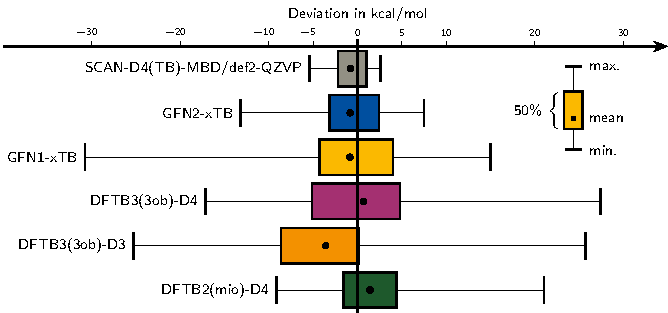
\includegraphics[width=\textwidth]{figures/s30l-boxplot.pdf}
  \caption{\label{fig:d4-s30l} Performance of different dispersion corrected
    tight binding methods on the S30L benchmark set, the values for SCAN-D4 are
    taken from Ref.~\cite{caldeweyher2019}.}
\end{figure}

To investigate the performance of the DFTB-D4 parameterizations we evaluate the
association energies for the S30L benchmark set~\cite{sure2015,brandenburg2018}.
DFTB-D4 is compared to DFTB3(3ob)-D3(BJ)~\cite{brandenburg2014},
GFN1-xTB~\cite{grimme2017} and GFN2-xTB~\cite{bannwarth2019}, additionally we
include the dispersion corrected SCAN~\cite{sun2015} functional for comparison
to DFT.  The deviation from the reference values is shown in
Fig.~\ref{fig:d4-s30l}. For the mio parameterization, complexes 4, 15 and 16
were excluded due to missing Slater--Koster parameters.  The direct comparison
of DFTB3(3ob)-D3(BJ) with a MAD of 7.1\;kcal/mol to the respective D4 corrected
method with a MAD of 6.5\;kcal/mol shows a significant improvement over its
predecessor. The DFTB2(mio)-D4 gives an improved description with a MAD of
4.5\;kcal/mol, which is better than GFN1-xTB with a MAD of 5.5\;kcal/mol. The
best performance is reached with GFN2-xTB due to the anisotropic electrostatics
and the density dependent D4 dispersion, giving a MAD of 3.6\;kcal/mol.


\paragraph{Tkatchenko-Scheffler (TS) dispersion}

The Tkatchenko-Scheffler correction (TS)~\cite{Tkatchenko2009} includes vdW
interactions as London-type atom-pairwise $C_6/R^6$-potentials with damping at
short inter-atomic separations, where the electronic structure method already
captures electron correlation. Suggested damping parameters for the mio and 3ob
parameter sets are listed in the supplementary material of
Ref.~\cite{hourahine-JCP-152-124101}. In the TS approach, all vdW parameters
including the static atomic dipole polarizability, $\alpha$, and
$C_6$-dispersion coefficients depend on the local electronic structure and the
chemical environment~\cite{Tkatchenko2009}. High-accuracy \textit{in vacuo}
reference values (below labeled by vac) are rescaled via
\begin{equation}
  x^2 = \left(\frac{\alpha_A^{\rm eff}}{\alpha_A^{\rm vac}}\right)^2 =
  \frac{C_{6,{\rm eff}}^{AA}}{C_{6,{\rm vac}}^{AA}}\:.
  \label{eq:MBDTS_effective_alphaC6}
\end{equation}
In the case of DFT, $x$ is approximated based on the Hirshfeld atomic
volumes~\cite{Hirshfeld1977}. When combined with DFTB, a fast yet accurate
alternative has been proposed~\cite{Stoehr2016} that does not require
evaluating a real-space representation of the electron density. Instead the
ratio between atom-in-molecule and \textit{in vacuo} net atomic electron
populations (i.e., $\tr\left(\rho\right)_A - Z_A$) are used to define $x$.

\paragraph{Many-body dispersion (MBD)}
Going beyond pairwise interactions, MBD~\cite{Tkatchenko2012,Ambrosetti2014}
accounts for many-atom interactions in a dipolar approximation up to infinite
order in perturbation theory. This is achieved by describing the system as a set
of coupled polarizable dipoles~\cite{Tkatchenko2012} with rescaled \textit{in
  vacuo} reference polarizabilities (as in
Eq.~\eqref{eq:MBDTS_effective_alphaC6}). At short-ranges this model switches,
via a Fermi-like function with a range of $\beta$, to the local atomic
environment as accounted for by solving a Dyson-like self-consistent screening
equation~\cite{Ambrosetti2014}. $\beta$ represents a measure for the range of
dynamic correlation captured by the underlying electronic structure method, so
depends on the density functional or DFTB parameterization. The recommended
$\beta$-values for the mio and 3ob parameter sets are listed in the
supplementary material of Ref.~\cite{hourahine-JCP-152-124101}.

\begin{figure}[htbp]
  \centering
  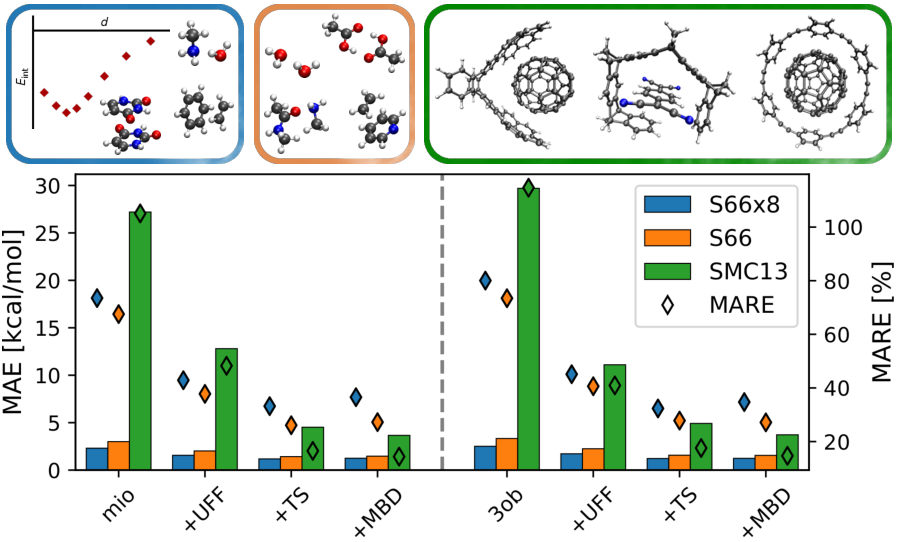
\includegraphics[scale=1.]{figures/DFTBvdW_benchmark_MAEs.pdf}
  \caption{\label{fig:dftbvdw_benchmarks} Mean absolute errors (MAE) and mean
    absolute relative errors (MARE) in inter-molecular interaction energies of
    bare DFTB and with different van der Waals models in comparison to
    high-level reference data. S66 and S66x8: small organic dimers and their
    dissociation curves~\cite{Rezac2011_S66,Rezac2011_S66x8}, SMC13: set of 13
    supra-molecular
    complexes~\cite{Ambrosetti2014_JPCL,Hermann2017,Stoehr2019_CSR}.}
\end{figure}
%
Fig.~\ref{fig:dftbvdw_benchmarks} and Ref.~\cite{Stoehr2016} demonstrate
that DFTB and MBD represent a promising framework to accurately study long-range
correlation forces and emergent behavior at larger length and time
scales. Recently, the DFTB+MBD approach has allowed the study of organic
molecular crystals~\cite{mortazavi2018} and solvated biomolecules, revealing the
complex implications of many-body vdW forces for proteins and their interaction
with aqueous environments~\cite{Stoehr2019}. Further improvements of TS and MBD,
including a better description of charge transfer effects~\cite{Gould2016} and
variational self-consistency~\cite{Ferri2015} may also be incorporated into DFTB
in the future.  Both methods are formulated independently of the underlying
electronic-structure methods. As a result \dftbp{} outsources the evaluation of
the MBD and TS interactions to Libmbd~\cite{libmbd}, an external open-source
library.


\subsection{Excited states and property calculations}

\subsubsection{Time dependent DFTB with Casida formalism}
\label{sec:TD-DFTB}

Electronic excited states are accessible in \dftbp{} through time dependent DFTB
methods (see Ref.~\cite{Niehaus2009} for a review and detailed
discussion of this formalism). In a linear response treatment in the
frequency domain, excitation energies are obtained by solving an eigenvalue
problem known as Casida or RPA (random phase approximation)
equations. Compared to first-principles time dependent DFT, the computational
scaling can be reduced in DFTB from $N^6$ to $N^3$. This is due to the Mulliken
approximation for two-electron integrals~\cite{Niehaus2001a}, which uses
transition charges $q^{pq\sigma}_A$,
\begin{equation}
  \label{qia}
  q_{A}^{pq\sigma} = \frac{1}{4} \sum_{\mu \in A}\sum_\nu  \left( c_{\mu
      p}^{\sigma} \tilde{c}_{\nu q}^{\sigma} +  c_{\mu q}^{\sigma}
    \tilde{c}_{\nu p}^{\sigma} + c_{\nu p}^{\sigma} \tilde{c}_{\mu
      q}^{\sigma} + c_{\nu q}^{\sigma} \tilde{c}_{\mu p}^{\sigma}
  \right), ~~ \tilde{\mathbf{c}}_p =  \mathbf{c}_p\cdot\mathbf{S},
\end{equation}
for transitions from Kohn-Sham orbital $p\sigma$ to $q\sigma$.

For fixed geometry, \dftbp{} provides a user defined number of low lying
excitation energies, oscillator strengths and orbital participations.  In
another mode of operation, the code computes excited state charges, eigenvectors
of the Casida equation and energy gradients for a specific state of interest,
which can be combined with MD or geometry relaxation. For spin-unpolarized
calculations, the response matrix is block diagonalized for the singlet and
triplet channels to speed up the computation.  \dftbp{} allows for the
computation of the excited state properties of systems with general fractional
occupation of the KS orbitals. This is useful, for example, for the simulations
of metals and semi-metals at finite temperature. For a detailed discussion on
spin-polarization and fractional occupation within TD-DFTB, see
Ref.~\cite{Dominguez2013}. The onsite correction, discussed in
Section~\ref{sec:onsite-correction}, is also possible for excited state
calculations and was shown to lead to marked improvements~\cite{Dominguez2013}.

Due to their improved treatment of charge-transfer transitions, range-separated
functionals are also relevant in the context of excited states. \dftbp{} implements
the TD-LC-DFTB method as described in Ref.~\cite{Kranz2017}. Compared to
conventional TD-DFTB, the lower symmetry of the response matrix leads to a
non-hermitian eigenvalue problem, which we solve by the algorithm
of Stratmann and co-workers~\cite{Stratmann1998}. Somewhat
surprisingly, it turns out that TD-LC-DFTB calculations are in practice not
significantly slower than TD-DFTB calculations (see Ref.~\cite{Kranz2017}
for a deeper discussion). Gradients can also be calculated with TD-LC-DFTB,
making it possible to perform geometry optimizations and MD simulations in
singlet excited states.

Please note that energetically high lying states and Rydberg excitations are
clearly outside of the scope of TD(-LC)-DFTB since their description generally
requires very diffuse basis sets. Apart from this class, the photochemically
more relevant set of low energy valence excitations are predicted with similar
accuracy to first principles TD-DFT, as several benchmarks
indicate~\cite{trani2011time,Dominguez2013,fihey2019performances}. As mentioned
above, charge-transfer excitations can now be also treated using
TD-LC-DFTB~\cite{Kranz2017}.

\subsubsection{SSR and excitations}
\label{para:ssrxc}

Currently, the SSR method implemented in \dftbp{} is formulated for active
spaces including two electrons in two fractionally occupied orbitals (i.e.,
SSR(2,2)) which is suitable for a singlet ground state and the lowest singlet
excited state as well as a doubly excited state~\cite{Lee19}. In addition, since
the SSR method is based on an ensemble representation and includes the
electronic correlation it can give correct state-interactions among nearly
degenerate electronic states. Thus, SSR approach is useful to investigate
conical intersections. The LC-DFTB/SSR method with scaled spin constants can
accurately describe the ground and excited states including $\pi/\pi*$ or
$n/\pi*$ character, undergoing bond cleavage/bond formation reactions as well as
the conical intersections where the conventional (TD)DFTB fails to obtain the
electronic properties. Analytic energy gradients as well as non-adiabatic
couplings are also available.


\subsubsection{Time-independent excited states from $\Delta$DFTB}

The linear response approach to excited-state properties in DFTB is efficient
and powerful, but there exist circumstances where a more direct route to excited
states is desirable. For example, excited-state properties obtained from linear
response theory require an additional order of derivatives relative to the
ground state. As noted in Section \ref{sec:TD-DFTB}, linear-response TD-DFTB
(like its parent method TD-DFT)~\cite{Dreuw2004} should invoke range-separation
to achieve a qualitatively correct picture of charge-transfer excitations and
related long-range phenomena~\cite{Kranz2017}.

As an alternative to the time-dependent linear-response approach, it is possible
to variationally optimize certain electronically excited states directly. The
$\Delta$DFTB method, modeled on the $\Delta$-self-consistent-field ($\Delta$SCF)
approach to excited states in DFT~\cite{Ziegler1977,Kowalczyk2011} involves
solving the SCC-DFTB equations subject to an orbital occupation constraint that
forces the adoption of a non-aufbau electronic configuration consistent with the
target excited state. This method is implemented for the lowest-lying singlet
excited state of closed-shell molecules in \dftbp{}~\cite{Kowalczyk2016}. The
converged, non-aufbau SCC-DFTB determinant is a spin-contaminated or ``mixed''
spin state, but the excitation energy can be approximately spin-purified through
the Ziegler sum rule which extracts the energy of a pure singlet from the
energies of the mixed state and the triplet ground state.

A significant advantage of the $\Delta$DFTB approach is that excited-state
gradients and hessians are quite straightforward to compute, both mathematically
and in terms of computational cost, relative to linear response
approaches. Benchmarks of $\Delta$DFTB excited-state geometries and Stokes
shifts~\cite{Kowalczyk2016} demonstrate the suitability of the method for
simulating excited-state energetics and dynamics of common organic chromophores
along the S$_1$ potential energy surface.

\subsubsection{Real-time propagation of electrons and Ehrenfest dynamics}

It is often desirable to study time dependent properties outside the linear
response regime, e.g. under strong external fields. The numerical propagation of
the electronic states enables the simulation of such phenomena and its coupling
to the nuclear dynamics in a semi-classical level can be included to lowest order
within the Ehrenfest method. Purely electronic (frozen-nuclei) dynamics as well
as Ehrenfest dynamics are included in \dftbp{}. We solve the equation of motion
of the reduced density matrix $\rho$ given by the Liouville-von Neumann equation
\begin{equation}
  \dot{\rho}=-\mathrm{i}\left(S^{-1} H[\rho] \rho-\rho H[\rho]
  S^{-1}\right)-\left(S^{-1} D \rho+\rho D^{\dagger} S^{-1}\right)
  \label{eq:rhodot}
  \text,
\end{equation}
with $D$ being the non-adiabatic coupling matrix $D_{\mu \nu} =
\dot{\mathbf{R}}_B \cdot \nabla_B S_{\mu \nu}$ and $\dot{\mathbf{R}}_B$ the
velocity of atom $B$. The on-site blocks can be calculated taking the
$\mathbf{R}_B \to 0$ limit, although neglecting those does not introduce
significant changes to the dynamics~\cite{Niehaus:2005da}.

Unitary evolution of $\rho$ with no change in its eigenvalues would require
$D^\dagger = -D$, which is normally not the case. Therefore, nuclear dynamics
can induce electronic transitions leading to
thermalization~\cite{Lin2009d}. Unitary evolution is recovered when all nuclear
velocities are equal (frozen-nuclei dynamics) and the second term in
Eq.~\ref{eq:rhodot} vanishes.

The force in the Ehrenfest-dynamics can be expressed
as~\cite{Todorov:2001ex,Niehaus:2005da}:
%
\begin{align}
  \mathbf{F}_A =& -\mathrm{Tr} \left\{ \rho \left( \nabla_A H^0 + \nabla_A S
  \sum_B \gamma_{AB} \Delta q_B + \nabla_A S S^{-1} H + H S^{-1} \nabla_A S
  \right) \right\} \nonumber \\ &- \mathrm{i} \; \mathrm{Tr} \left\{ \rho
  \nabla_A S S^{-1} D + \mathrm{h.c.} \right\} + \mathrm{i} \; \sum_{\mu \nu}
  \left\{ \rho_{\nu \mu} \langle \nabla_A \phi_{\mu} | \nabla_B \phi_{\nu}
  \rangle \cdot \dot{\mathbf{R}}_B + \mathrm{h.c.} \right\} \nonumber \\ &-
  \Delta q_A \sum_{B} \nabla_A \gamma_{AB} \Delta q_B - \nabla_A E_{rep} -
  \Delta q_A \mathbf{E}(t),
  \label{eq:ehrenforces}
\end{align}
where $\mathbf{E}(t)$ is the external electric field. In the present
implementation, the velocity dependent terms have been neglected, they would
vanish for a complete basis~\cite{Niehaus:2005da} and are necessary for momentum
but not for energy conservation~\cite{Todorov:2001ex}.  When the system is
driven externally by an electric field, a dipole coupling term is added in the
time-dependent hamiltonian in Eq.~\ref{eq:rhodot}.

Some applications that have been enabled by the speedup over time-dependent DFT
are the simulation of the plasmon-driven breathing-mode excitation in silver
nanoparticles of 1-2~nm in diameter~\cite{Bonafe2017a} and the simulation of
transient absorption pump-probe spectra in
molecules~\cite{Bonafe2018,Hernandez2019}.

Whenever a time propagation approach is used for the calculation of absorption
spectra in the linear regime, this method is equivalent to calculations using
the Casida formalism and shares its strengths and limitations. Specific pitfalls
of the time dependent approach come into play whenever simulating the response
to intense external fields. In these cases the poor description of highly lying
excited states due to the use of a minimal basis set would likely be inaccurate
if these states are populated during the dynamics.

\subsubsection{pp-RPA}

An approximate particle-particle RPA scheme, the so called
pp-DFTB~\cite{Kranz2017}, is now implemented in DFTB+. Particle-particle RPA,
based on the pairing matrix fluctuation formalism, has been shown to be an
efficient approach for the accurate description of double and charge-transfer
(CT) excitations involving the highest occupied molecular orbital (HOMO) (see
Ref.~\cite{Yang2017} for details).  In Ref.~\cite{Kranz2017} we
compare against TD-LC-DFTB for CT excitation energies of donor-acceptor
complexes. TD-LC-DFTB has the advantage that transitions do not necessarily have
to involve the HOMO of the system. Alternatively pp-DFTB does not require
parameter tuning and is efficient for the lowest lying excitations.

Although one of the strengths of the original pp-RPA formulation lies on the
accurate description of Rydberg excitations, our approximate formalism based on
DFTB fails to describe these kind of transitions, as explained above in
section~\ref{sec:TD-DFTB}.

\subsubsection{Coupled perturbed responses}

\dftbp{} supports several types of response calculations for second-order
derivatives. The general form of the response evaluation is via standard
perturbation theory:
\begin{align}
  P_{ij} &= \mel**{c_i}{H^{(1)}_{ij} - \epsilon_j S^{(1)}_{ij}}{c_j}\\
  \epsilon_i^{(1)} &= P_{ij} \delta_{ij}\\
  U_{ij} &= P_{ij} / \left( \epsilon_j - \epsilon_i \right)\\
  c_i^{(1)} &= \sum_j U_{ij} c_j^{(0)}\\
  \rho^{(1)} &= \sum_i n^{(1)}_i \dyad{c^{(0)}} + \sum_i n^{(0)}_i \left(
               \dyad{c^{(1)}}{c^{(0)}} + \qcc\right),
\end{align}
where the sums for the states that $U$ mixes together may be over all states, or only
the virtual space (parallel gauge) depending on application. $U$ is either
anti-symmetric (hermitian) or has no symmetry depending on whether the derivative
of the overlap matrix is non-zero.

In the case of systems with degenerate levels, a unitary transformation, $Z$, that
diagonalizes the block of $P$ associated with that manifold can be applied to
the states, note that this sub-block is always symmetric (hermitian), leading to
orthogonality between states in the perturbation operation:
\begin{align}
  \tilde{P}_{ij} &= z_{ik} P_{kl} z_{li}^\dag\\
  \tilde{c}_i &= c_j z_{ji}
\end{align}

For fractionally occupied levels, the derivatives of the occupations for
$\mathbf{q}=0$ perturbations (where change in the Fermi energy should be
included) are then evaluated~\cite{nishimoto2017317}.

Time dependent perturbations at an energy of $\hbar \omega$ can be written as
\begin{align}
  U_{ij}^\pm &= P_{ij} / \left( \epsilon_j - \epsilon_i \pm \hbar \omega + i\eta
               \right)\\
  c_i^{(1)\pm} &= \sum_j U_{ij}^\pm c_j^{(0)}\\
  \rho^{(1)} &= \sum_i n^{(1)}_i \dyad{c^{(0)}} + \sum_i n^{(1)}_i \dyad{c^{(0)}}
               + \sum_\pm \sum_i n^{(0)}_i \left( \dyad{c^{(1)\pm}}{c^{(0)}} + \qcc \right).
\end{align}
Here the small constant $\eta$ prevents divergence exactly at excitation
poles.

Derivatives with respect to external electric fields and potentials are included
(giving polarizabilities and dipole excitation energies), with respect to atom
positions (at $\mathbf{q}=0$, providing Born charges and electronic derivatives
for the hessian) and with respect to $k$ in periodic systems (effective masses
and also the Berry connection via $\braket{u}{\sfrac{\partial u}{\partial
    \mathbf{k}}}$). In the longer term, perturbation with respect to magnetic
fields, boundary conditions (elastic tensors) and alternative approaches
(Sternheimer equations for $\mathbf{q}\ne0$, and also lower computationally scaling
density matrix perturbation theory) are planned.

\subsection{Non-equilibrium Green's function based electron transport}

Electron transport in the steady-state regime is described in \dftbp{} within a
non-equilibrium Green's function (NEGF) method~\cite{pecchia2004, haug2008} as
implemented in the code-independent libNEGF~\cite{libnegf-repo} library.  The
density matrix is evaluated in terms of the electron-electron correlation matrix
$G^{<}$~\cite{haug2008},

\begin{equation} \label{negf1}
  \rho = \frac{1}{2\pi \mathrm{i}} \int_{-\infty}^{+\infty} {G^{<}(E)
    \mathrm{d}E}.
\end{equation}
%
Open boundary conditions are included in terms of electron baths with an
arbitrary spectrum and chemical potential, allowing for a seamless description
of charge injection from electrodes with an applied bias. The density matrix is
then used to evaluate a real-space electron density distribution which is
coupled self-consistently with a Poisson solver.  We perform a full band
integration of Eq.~\ref{negf1}, utilizing a complex contour integral to reduce
the number of integration points~\cite{pecchia2004}. This allows for an implicit
description of dielectric properties which is crucial for an accurate modeling
of ultra-scaled electron devices~\cite{markov2015,chu2018}. After
self-consistency is achieved, the total current flowing in the system is
calculated with the Landauer/Caroli formula for the non-interacting case, or
with the Meir-Wingreen formula for the interacting case~\cite{haug2008}. A
detailed description of the numerical algorithms and self-consistent coupling is
presented in Ref.~\cite{pecchia2008}. Here we summarize the main features
which might differentiate \dftbp{} from other nano-device simulation packages:
(i) support for $N \geqslant 1$ electrodes (enabling structures from surfaces
and semi-infinite wires to multiple terminal geometries), (ii) $O(L)$
memory and time scaling (where $L$ is the system length) via a block-iterative
algorithm, (iii) a real space Poisson solver with support for gates and
dielectric region and (iv) evaluation of local currents.  Being a parameterized
tight binding method, its usage is bounded by the availability of good
parameters for the system under investigation.

\begin{figure}[htbp]
  \centering
  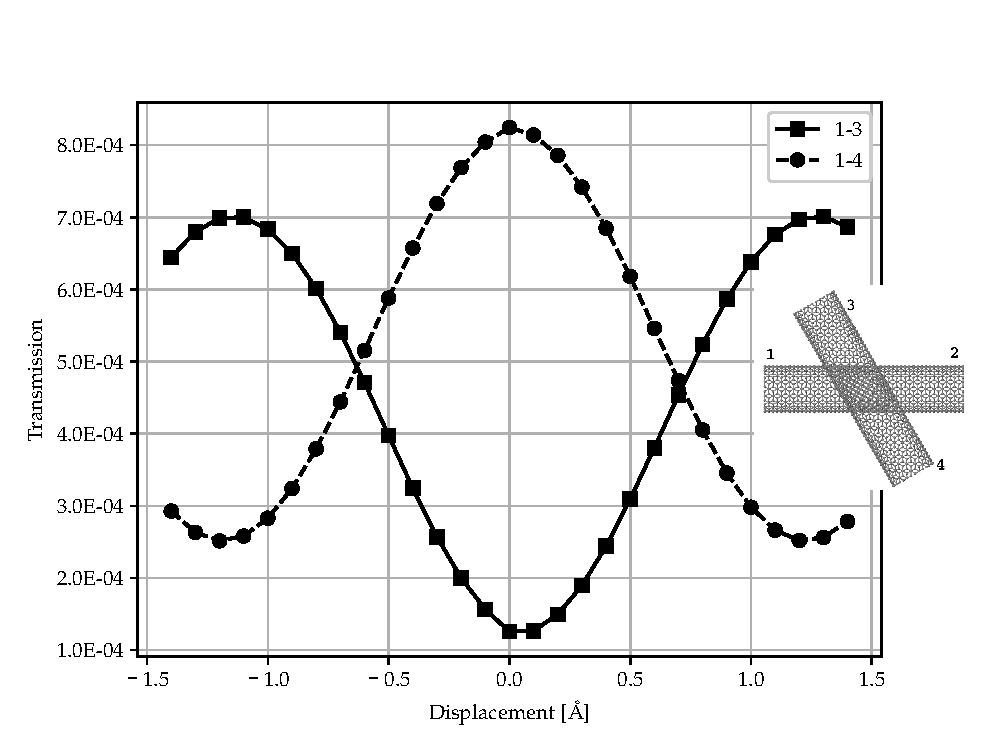
\includegraphics[scale=.75]{figures/dftb-negf1.eps}
  \caption{\label{fig:dftb_negf1} Transmission across two (10,10) CNTs as a
    function of the displacement of the top CNT along the axis of the bottom
    CNT. The two curves represent the transmission resolved between the
    electrode 1 of the bottom CNT, and respectively electrodes 2 and 3 of the
    top CNT (as labeled in the figure in inset).}
\end{figure}

Carbon-based materials and molecular junctions have been a typical use-case
since the first integration of DFTB and NEGF~\cite{reimers2007, latessa2005,
  penazzi2013}. In Fig.~\ref{fig:dftb_negf1} we show a non-SCC calculation
example of transmission in linear response for a multi-terminal device. The
simulated system is a cross-junction between two (10,10) Carbon nanotubes
(CNTs). One CNT is tilted by 60$\degree$ with respect to the second and the
transmission is calculated by displacing one CNT along the axis of the other. The transmission follows, as expected, a periodic pattern in accordance with
the lattice repeat of 0.25~nm along the axis of the CNT.

Currently we are working on extending transport functionality in \dftbp{} with
electron-phonon coupling~\cite{pecchia2004b, pecchia2007, penazzi2016,
  gagliardi2008}, electron-photon coupling, spin polarized transport and phonon
transport~\cite{medrano15b, medrano16, Martinez19, MedranoRev}.

Overall, DFTB-NEGF shares many similarities with DFT based implementations, and
it also inherits some shortcomings the less experienced users should be aware
of. For example, the open boundary treatment demands that external and
non-equilibrium potentials are screened at the boundaries~\cite{haug2008}.
Therefore, the simulated system should be large enough compared to the screening
length.  This condition is easily achieved with bulk metallic electrodes, but it
can be difficult with low dimensional systems which exhibit poor screening. When
this condition is not fulfilled, unphysical discontinuities in the potential may
be obtained. Also, compared to band structure calculations, NEGF tends to
converge with more difficulty~\cite{ozaki2010}. Aside from these common
challenges, it is important that for DFTB-NEGF calculations any set of
parameters should be evaluated by verifying at the least band structure
properties in the energy range of interest. DFTB parameters fitted to reproduce
total energies and forces might be excellent in those application but lack the
necessary accuracy in the band structure. Depending on the degree of accuracy
required, an {\it ad hoc} fitting for transport calculations could also be
necessary, as for example in the case of silicon~\cite{markov2015b}.

\subsection{Extended Lagrangian Born-Oppenheimer dynamics}

The Extended Lagrangian Born-Oppenheimer molecular dynamics (XLBOMD) framework
allows~\cite{ANiklasson08, ANiklasson17} molecular dynamics on the
Born-Oppenheimer surface with only one hamiltonian diagonalization per time step without the
need for self-consistency cycles.  The basic idea is based on a backward error
analysis, i.e.\ instead of calculating approximate forces through an expensive
non-linear iterative optimization procedure for an underlying exact potential
energy surface, XL-BOMD calculates exact forces for an approximate ``shadow'' potential energy surface, $U({\bf R},n)$. This is approximated from a
constrained minimization of a linearized Kohn-Sham energy functional~\cite{ANiklasson14,ANiklasson17}. The functional is linearized around an
approximate ground state density, $n$. This density is included as a dynamical
field variable driven by an extended harmonic oscillator centered on an approximate ground state, $q[n]$, which is given by the minimization of the linearized Kohn-Sham functional. The harmonic well is
defined in terms of a metric tensor, $T = K^T K$, where the kernel $K$ is
assumed to be the inverse Jacobian of the residual function, $q[n] - n$~\cite{ANiklasson17}.  The equations of motion are given by
\begin{equation}
  M_I{{\bf \ddot R}}_I = -\left. \frac{\partial U({\bf R},n)}{\partial
    R_I}\right \vert_n \quad \text{and} \quad {\ddot n} = -\omega^2 K(q[n] - n).
\end{equation}
Here $M_I$ are the atomic masses, ${\bf R}_I$ are the nuclear coordinates, $\omega$ the frequency of the harmonic oscillator, $q[n]$ are the net Mulliken charge vectors (from an optimized linearized energy expression), and $n$ is the extended dynamical
variable that is set to the optimized ground state net Mulliken charge vector in
the initial time step. Details of the \dftbp{} implementation are given in
Ref.~\cite{BAradi15}.

We currently approximate the kernel by a scaled
identity matrix,
\begin{equation}
  K = -cI, ~~ c\in [0,1].
\end{equation}
For many problems this is a sufficiently accurate approximation. However, for
the most challenging problems including simulations of reactive chemical systems
or metals, the scaled delta function is not a sufficiently stable
approximation. Improved approximations have been developed~\cite{ANiklasson17}
and will be implemented in the \dftbp{} program in the near future.

\subsection{Objective geometries}

Objective structures~\cite{James2006} (OS) describe geometries consisting of a
set of identical cells, where corresponding atoms in different cells can be
mapped onto each other by orthogonal transformation(s). Both finite and infinite
OS are possible. Currently we describe
structures~\cite{James2006,Dumitrica2007,ZhangHuaDumitrica2008}
possessing $C_n$ rotational symmetry and a $C_m \otimes T$ screw axis, where $n
\in \mathbb{N}^{*}$ and $m \in \mathbb{R}^{+}$:
\begin{equation}
  \mathbf{X}_{i, \zeta, \xi} =
  \left(C_n\right)^\xi \left(C_m\right)^\zeta \mathbf{X}_{i}+ T^\zeta\qc{i \in N},
  \label{basic_replicate_obj}
\end{equation}
with $N$ atoms in the reference objective cell ($\{\mathbf{X}_i\}$) and
$\left\{\zeta,\xi\right\} \in \mathbb{N}$ where $-\infty < \zeta < \infty$ and
$0 < \xi < n$. Exploiting the objective boundary conditions (OBCs) can introduce
substantial computational savings, for example irrational values of $m$ lead to
structures with a small OS cell but an infinitely long one dimensional periodic
boundary condition (PBC), i.e.\ intractable purely as a $T$ operation. OBCs
generalize symmetry-adapted Bloch sums for orbitals. As with molecular and
periodic structures~\cite{aradi-jpca-2007}, most expressions in \dftbp{} can be
performed in real space, via the boundary-condition agnostic and sparse
representation of matrices in real space, only solution of the hamiltonian
requires dense matrices and $k$-points. For the long-range coulombic and
dispersion interactions in DFTB we also require lattice sums that are
generalized to these boundary conditions~\cite{Nikiforov2013}.

Further examples can be found in Refs.~\cite{Nikiforov2014,
  XU2019, DUMITRICA2019}, but here we demonstrate the
\begin{figure}[htbp]
  \begin{center}
    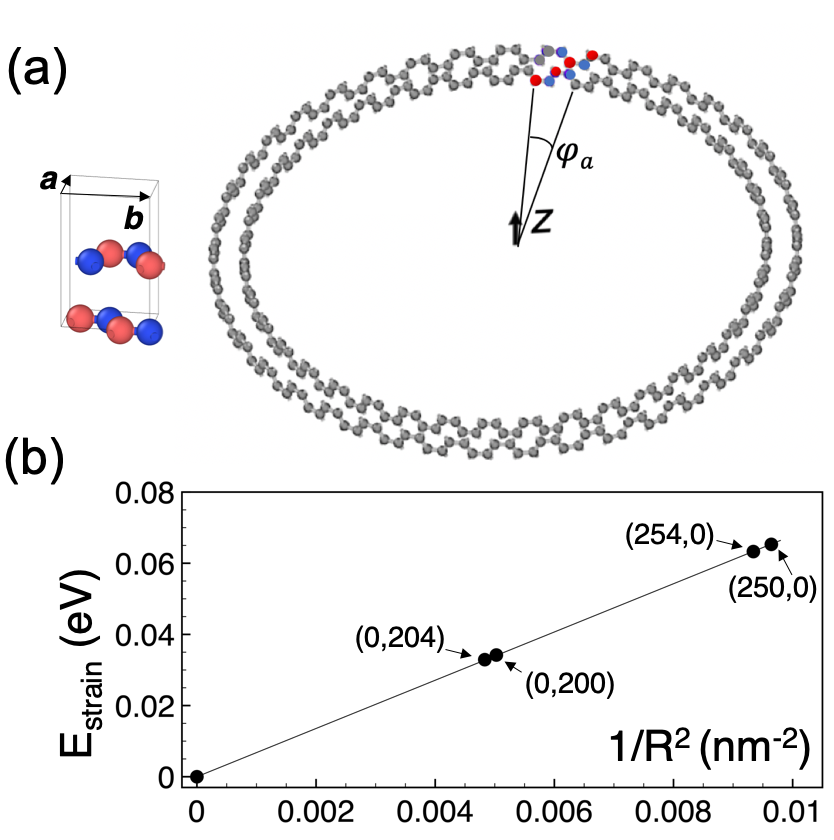
\includegraphics[scale=0.4]{Fig2_td.png}
    \caption{\label{fig2_td} (a) OS of a \ce{BN} bi-layer tube with a \ce{B4N4}
      unit (red and blue atoms). Angular, but not translational, objective
      images are shown in gray. (b) Bending energy (circles)
      versus curvature with a linear fit.}
  \end{center}
\end{figure}
bending of a \ce{BN} bi-layer. Figure~\ref{fig2_td} shows a double-walled
tubular OS with curvature of $1/R$ (from the tube radius) that
represents the bent bi-layer. Bending along the ${\bf a}$ (${\bf b}$) direction of the
sheet is an `armchair' (`zig-zag') tube with a $C_n$ proper axis, described as
an 8 atom objective cell in which we select {\bf T}=${\bf a}$ ({\bf T}=${\bf
  b}$) and no tube twist.  The bi-layer bends as a plate, with the outer wall
stretching and the inner compressing along their circumferential directions; its
energy change is interpreted as bending strain ($E_\text{bend}$). It is important
to note that the corresponding curvature is not an imposed constraint but a
result of the calculation: $R$ is the average tube
radius. Figure~\ref{fig2_td}(b) demonstrates linearity with bending, fitting to
$E_\text{bend}=(1/2)D(|{\bf a}| |{\bf b}|)(1/R)^2$ gives a bi-layer bending
constant of $D=120$~eV.

A wider range of OS will be made available in later \dftbp{}
releases, along with adapted electrostatic evaluation for these structures.

\subsection{Extended Tight Binding hamiltonian}

The extended tight binding~(xTB) methods were primarily designed for the fast
calculation of structures and non-covalent interaction energies for finite
systems with a few thousand atoms. The main parameterizations, GFN\textit n-xTB,
target molecular geometries, frequencies and non-covalent interactions following
mostly a global and element-specific parameter only strategy. The historically
first parameterization, GFN1-xTB, covers all elements up to $Z=86$ and is now
supported in \dftbp{}. Its successor, GFN2-xTB~\cite{bannwarth2019}, will also be
made available in the future.

We briefly outline the xTB methods, for a more detailed discussion and
comparison to other methods we refer to
Refs.~\cite{grimme2017,bannwarth2019}.  The xTB core hamiltonian is
constructed in a partially polarized STO-\textit nG basis set with diagonal
terms made flexible by adding a dependence on the local chemical environment
according to a coordination number (CN), similar to that used in
DFT-D3~\cite{grimme2010}:
%
\begin{equation}
  H_{\lambda\lambda} = H^l_A - H^l_{{CN}_{A}} {CN}_{A}.
\end{equation}
%
The off-diagonal terms are approximated as an average of the diagonal terms
proportional to the overlap between the corresponding basis functions.

Both GFN1-xTB and GFN2-xTB include density fluctuation up to a third order
diagonal terms, while the distance dependence of the Coulomb interaction within
the isotropic second order term is described by a generalized form of the
Mataga--Nishimoto--Ohno--Klopman~\cite{klopman1964,ohno1964,mataga1957}
expression. In GFN2-xTB the expansion of the second order density fluctuations
goes beyond the usual isotropic energy terms and includes interactions up to
$R^{-3}$, i.e., charge--dipole, dipole--dipole and charge--quadrupole
interactions, which significantly improves the description of inter-molecular
interactions, like halogen bonds and hydrogen bonds, without the need to
include force-field-like corrections as in DFTB or GFN1-xTB. It is planned to implement full multipole electrostatics with Ewald summation
in \dftbp{} to enable GFN2-xTB and other generalized DFTB
models~\cite{Bodrog2012}.

GFN1-xTB and GFN2-xTB have been extensively tested for their target
properties~\cite{bannwarth2019}, further studies regarding structures for
lanthanoid complexes~\cite{bursch2017} and transition metal
complexes~\cite{bursch2019} have shown xTB methods to be robust for all its
parameterized elements.  Errors in this methods are very systematic, which can
be used to devise correction schemes for off-target properties like reaction
enthalpies~\cite{kromann2018}.

\subsubsection{Outlook}

In recent years machine learning has been utilized with \dftbp{}, usually to
enhance the generation and description of the repulsive
potentials~\cite{Knaup2007, Kranz2018, Zhu2019, Huran2018, Goldman2018} or try
to improve on electronic parameters~\cite{Li2018, Huran2018}. Related
$\Delta$-machine learning~\cite{Ramakrishnan2015} methodologies based on neural
network corrections for DFTB energies and forces have been also reported
recently~\cite{Shen2016, Shen2018}. We are currently in the process of developing
a new unified machine-learning framework, which for a target system allows
optimal adaption of both the electronic and the repulsive contributions. Given
the predicted DFTB model, one would still have to solve it in order to obtain
the system properties. On the other hand, changing external conditions
(temperature, electric field, applied bias, etc.) would not require additional
training in this approach, and also long range effects (e.g. metallic states)
could be described easily.


\section{Technical aspects of the \dftbp{} package}


\subsection{Parallel scaling}

In large-scale simulations the solution of the DFTB hamiltonian to obtain the
density matrix eventually becomes prohibitively expensive, scaling cubically
with the size of the system being simulated. The diagonalization infrastructure
in \dftbp{} has undergone a major upgrade, including distributed parallelism and
GPU accelerated solutions to address this cost. If instead the density matrix is
directly obtained from the hamiltonian, circumventing diagonalization, then
linear or quadratic scaling can now be obtained, depending on the chosen method.
\dftbp{} will continue to benefit from developments in these advanced solvers as
we move into the era of exascale computing.


\subsubsection{The ELSI interface and supported solvers}
\label{sec:elsi}

ELSI~\cite{elsi_yu_2018} features a unified software interface that
simplifies the use of various high-performance eigensolvers,
(ELPA~\cite{elpa_marek_2014}, EigenExa~\cite{eigenexa_imamura_2011},
SLEPc~\cite{slepc_hernandez_2005} and
MAGMA~\cite{magma_dongarra_2014}) and density matrix solvers
(libOMM~\cite{libomm_corsetti_2014}, PEXSI~\cite{pexsi_lin_2013} and
NTPoly~\cite{ntpoly_dawson_2018}). We convert the sparse \dftbp{} $H$
and $S$ structures~\cite{aradi-jpca-2007} into either standard 2D
block-cyclic distributed dense matrices or sparse 1D block distributed
matrices compatible with the ELSI interface. All $k$-points and spin
channels are then solved in parallel.

The ELSI-supported solvers, when applied in appropriate cases, can lead to a substantial
speedup over the default distributed parallel diagonalization method in \dftbp{}, i.e.,
eigensolvers in the ScaLAPACK
library~\cite{scalapack_blackford_1997,dc_tisseur_1999,mrrr_vomel_2010}.
Figure~\ref{fig:solvers} demonstrates two examples: Non-self-consistent-charge,
spin-non-polarized, $\Gamma$-point calculations for a \ce{C64000} nanotube (CNT)
and a \ce{Si6750} supercell, with 25600 and 27000 basis functions, respectively.
\begin{figure*}[htbp]
  \centering
  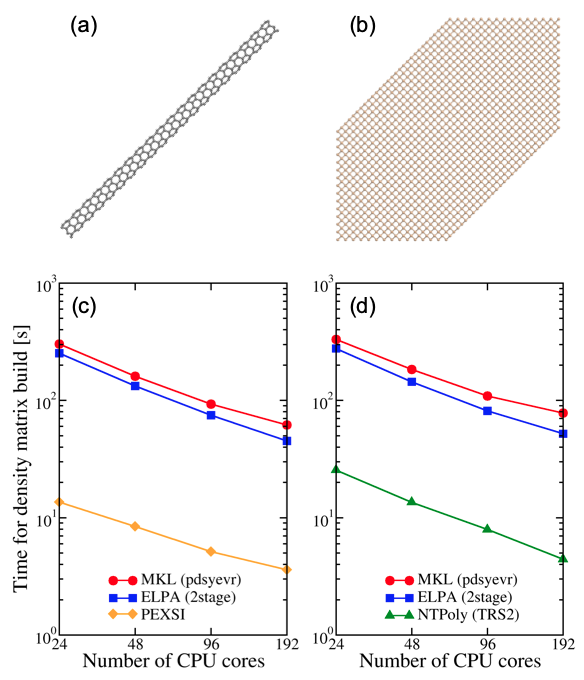
\includegraphics[width=0.5\textwidth]{figures/solvers.png}
  \caption{Atomic structures of (a) the carbon nanotube (CNT) model (6400
    atoms) and (b) the silicon supercell model (6750 atoms). The length of the
    actual CNT model is 16 times that of the structure shown in (a). (c) and (d)
    show the time to compute the density matrix for model (a) and (b),
    respectively. Calculations are performed on the NewRiver computer. MKL
    pdsyevr and ELPA2 first compute all the eigenvalues and eigenvectors of the
    eigensystem of $H$ and $S$, then build the density matrix. PEXSI and NTPoly
    directly construct the density matrix from $H$ and $S$.}
  \label{fig:solvers}
\end{figure*}
Figure~\ref{fig:solvers} (c) shows the time to build the density matrix for the
CNT model with three solvers, the pdsyevr eigensolver in the MKL implementation
of ScaLAPACK, the ELPA2 eigensolver and the PEXSI density matrix solver. Here
both the MKL's version of pdsyevr eigensolver and the ELPA2 eigensolver adopt a
two-stage tri-diagonalization
algorithm~\cite{2stage_bischof_1994,elpa_marek_2014,mkl_arturov_2018}. In terms
of performance, ELPA2 and MKL pdsyevr are similar, while both are outperformed
by the PEXSI solver by more than an order of magnitude. The
PEXSI~\cite{pexsi_lin_2013} method directly constructs the density matrix from
the hamiltonian and overlap matrices with a computational complexity of
$O(N^{\sfrac{(d+1)}{2}})$ for $d=1\ldots3$D systems. This reduced scaling
property stems from sparse linear algebra, not the existence of an energy
gap. Therefore, for any low-dimensional system, regardless of electronic
structure, PEXSI can be used as a powerful alternative to diagonalization. A
similar comparison of solver performance for the silicon supercell model is
shown in Fig. \ref{fig:solvers} (d), where the NTPoly density matrix solver
shows greater performance than the MKL pdsyevr and ELPA2 eigensolvers. Around
its massively parallel sparse matrix multiplication routine, NTPoly implements
various linear scaling density matrix purification methods, including the
$2^\text{nd}$ order trace-resetting purification method
(TRS2)~\cite{ANiklasson02} used here. While PEXSI is not
particularly suited for 3D systems, NTPoly offers an alternative as long as the
system has a non-trivial energy gap.

\subsection{GPU computing}

Graphics processing unit (GPU) acceleration is implemented in \dftbp{}. Given
the nature of the underlying theory, the time-limiting step in routine
calculations corresponds to the diagonalization of the hamiltonian matrix,
taking in the order of 90-95\% of the total running time. The hybrid CPU--GPU
implementation in \dftbp{} replaces the LAPACK-based eigensolver with a GPU
eigensolver based on the divide-and-conquer algorithm as implemented in
MAGMA~\cite{TOMOV2010232}.

Benchmarking of the code shows that at least 5000 basis functions are necessary
to exploit the power of the GPUs and to produce an observable speedup with
respect to the CPU-only code. For systems spanning a vector space comprised of
70000 basis functions, speedups of $17\times$ have been observed in a system
with 6 NVIDIA\textsuperscript{\textregistered}
Tesla\textsuperscript{\textregistered} V100 with respect to the multi-threading
CPU-only implementation (see Fig.~\ref{fig:gpu}).

\begin{figure}[htbp]
  \centering
  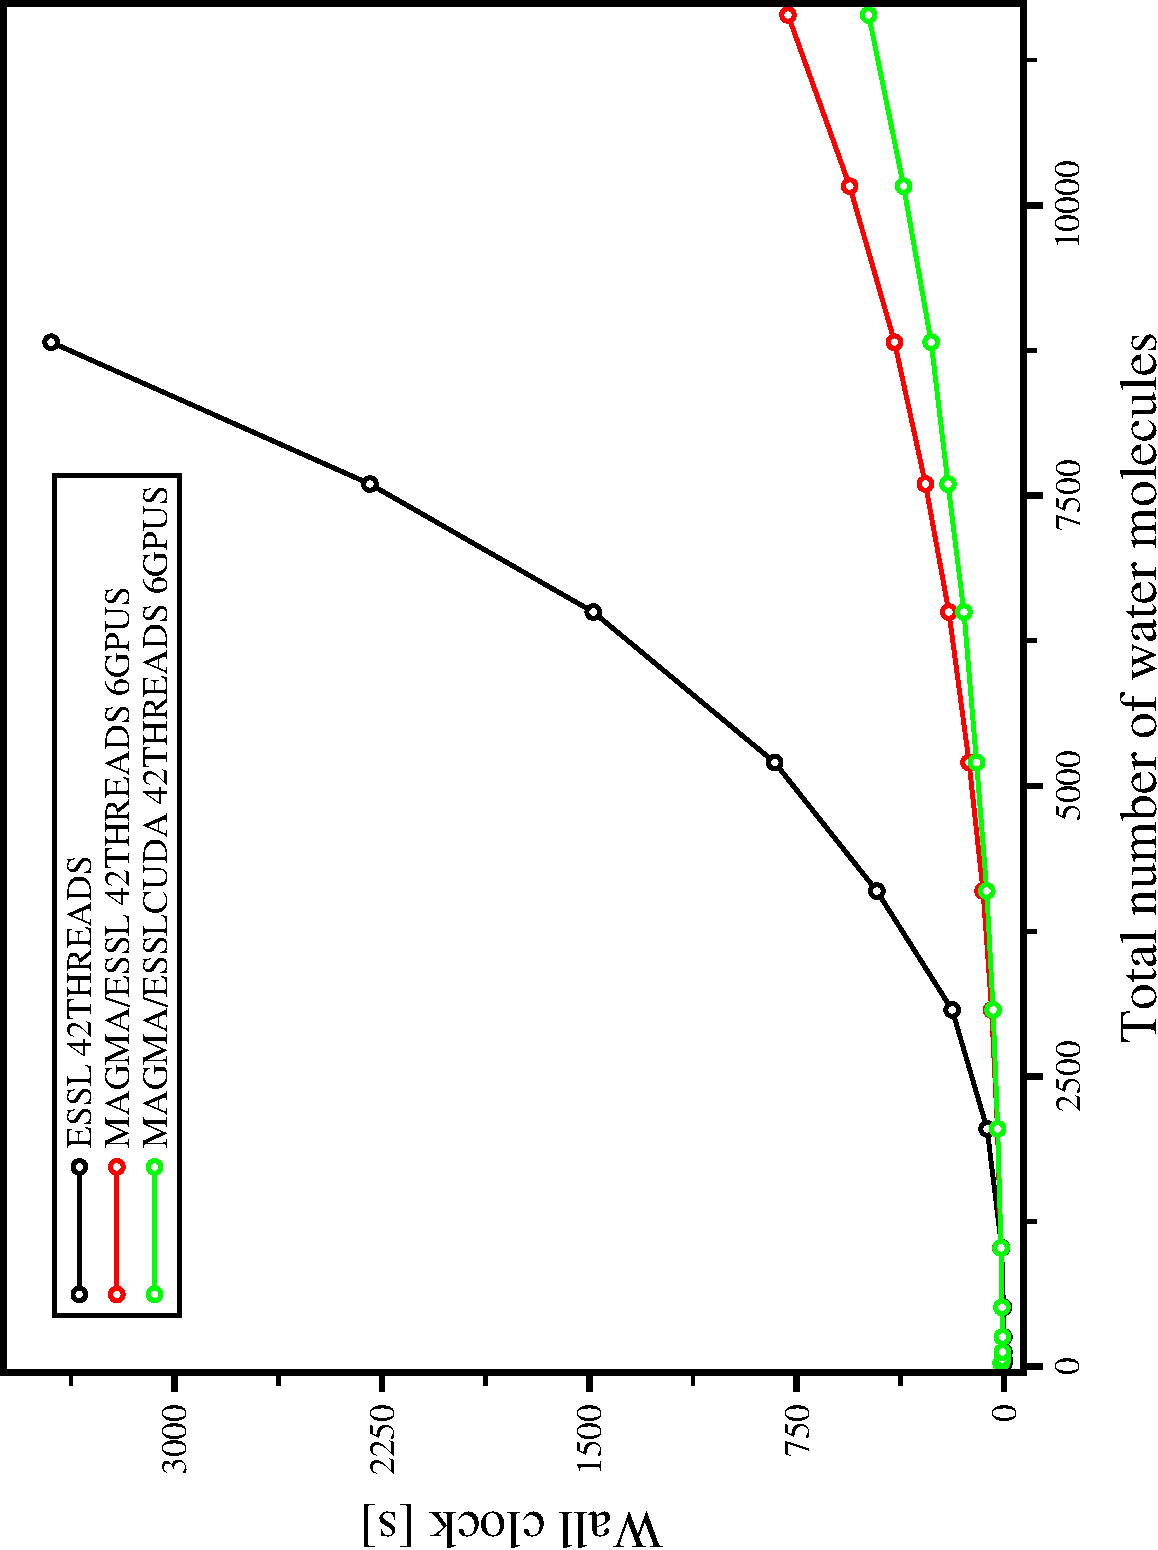
\includegraphics[width=8cm,angle=270]{summit-h2o.pdf}
  \caption{Wall clock running times for total energy calculations of water
    clusters (with 6 basis function / water molecule). The black curve shows
    timings obtained using the LAPACK compatible ESSL eigensolver on the CPU,
    the red/green curves show timings obtained using the MAGMA and the ESSL
    libraries without/with ESSL-CUDA off-loading. Timings has been made on the
    Summit machine using 42 threads for 42 physical cores.}
  \label{fig:gpu}
\end{figure}


\section{Interfacing \dftbp{} with other software packages}

\dftbp{} can be currently interfaced with other software packages using three
different ways of communications: file communication, socket based, or direct
connection via the \dftbp{} API as a library. The first one is very easy to
implement but comes with an overhead for the file I/O, while the latter two
enable more efficient coupling at the price of somewhat higher complexity in
implementation.

\subsection{File based communication}

When using file based communication, the external driver creates necessary input
files and starts an individual \dftbp{} program for each of the
inputs. After \dftbp{} has finished, the driver analyses the created output
files and extracts the necessary information from those. \dftbp{} had been
interfaced using file based communication to, among others, the
phonopy~\cite{phonopy} code for finite difference harmonic and anharmonic phonon
calculations and the Atomic Simulation Environment (ASE)
package~\cite{larsen-jpcm-2017} (a set of tools and Python modules for setting
up, manipulating, running, visualizing and analyzing atomistic simulations).

\subsection{Socket interface}

The i-PI~\cite{ipi} interface for communication with external driving codes is
supported by \dftbp{}. \dftbp{} can then be driven directly instead of
using file I/O. The initial input to \dftbp{} specifies the boundary conditions,
type of calculation and chemical information for atoms, the code then waits to
be externally contacted. This kind of communication with \dftbp{} can be used
by, among others, the i-PI universal force engine package~\cite{ipi} and
ASE~\cite{larsen-jpcm-2017}.


\subsection{\dftbp{} library, QM/MM simulations}

\subsubsection{Gromacs integration}

DFTB quantum-chemical models may be utilized as a QM engine in hybrid
quantum-mechanical / molecular mechanical (QM/MM) approaches.  This allows for
example efficient simulations of chemical processes taking place in bio-molecular
complexes.  The \dftbp{} library interface has been connected to the
Gromacs~\cite{Gromacs7} MM-simulation software package. (The Gromacs part of the
integration is contained in a fork of the Gromacs main
branch~\cite{gromacs-dftbplus-repo}) At the start of the simulation, the \dftbp{}
input file is read in, and a DFTB calculation environment is created, containing
all of the necessary information (parameters), but no atomic coordinates yet.
In every step of MD simulation or of energy minimization, the calculation of
forces starts with a call to the \dftbp{} API, passing the coordinates of QM
atoms and the values of electrostatic potentials induced by the MM atoms at the
positions of the QM atoms.  \dftbp{} then returns QM forces and QM charges back
to Gromacs, where the QM/MM forces are calculated in the QM/MM routines.
Gromacs then continues by calculating the MM forces, integration of equations of
motion etc.

Sometimes the electrostatic interactions can not be represented as an external
potential but depend also on the actual values of the QM-charges (i.e.,
polarizable surroundings). In those cases a callback function can be
passed to \dftbp{}, which is then invoked at every SCC iteration to update the
potential by the driver program whenever the QM charges
change. In the \dftbp{}/Gromacs integration we use this technique to calculate
the QM-QM electrostatic interactions in periodic systems with the highly
efficient Particle Mesh Ewald method~\cite{Darden1993} implemented in Gromacs.

\subsubsection{DL\_POLY\_4 integration with MPI support}

DL\_POLY\_4 is a general-purpose package for classical molecular dynamics (MD)
simu\-la\-tions~\cite{dl_poly2006}. In conjunction with the recent extension of
\dftbp{}'s API, DL\_POLY\_4.10 supports the use of \dftbp{} for self-consistent
force calculations in place of empirical force fields, for Born-Oppenheimer
molecular dynamics.

The interface fully supports passing MPI communicators between the programs,
allowing users to run simulations in parallel, across multiple processes. The
MPI parallelization schemes of DL\_POLY\_4 and \dftbp{} differ
considerably. DL\_POLY\_4 utilizes domain decomposition to spatially distribute
the atoms which comprise the system across multiple processes, whereas \dftbp{}
distributes the hamiltonian matrix elements using BLACS decomposition. This does
not impose any serious restrictions as DL\_POLY\_4 and \dftbp{} run
sequentially, with \dftbp{} being called once per MD time step.

The DL\_POLY\_4 - \dftbp{} interface works by gathering the atoms from each
DL\_POLY\_4 process, such that all processes have a complete copy of all the
atoms. Coordinates, species types and the atomic ordering are then passed to
\dftbp{}.  The calculated forces are returned to DL\_POLY\_4, which
redistributes them according to its domain decomposition and the atomic
positions are propagated one time step.

Spatial decomposition means that atoms can propagate between processes. Because
atoms are gathered sequentially according to their process id (or rank), when
atoms propagate between processes their ordering effectively changes. The
\dftbp{} API facilitates this and is therefore able to support any molecular
dynamics software that implements domain decomposition parallelization, however,
the total number of atoms (and atom types) must be conserved during the
simulation.

\subsection{Meta-dynamics using Plumed}

Molecular dynamics is often plagued by high energy barriers that trap the
nuclear ensemble in one or several local minima. This leads to inefficient or
inadequate sampling of the ensemble and thus inaccurate predictions of
physicochemical properties~\cite{RN1,RN2,RN3}. This `timescale' problem is
typical for rare-event systems, or those in which ergodicity of a particular
state is impeded by the local topology of the potential energy surface. A
variety of methods have been conceived to circumvent this, including
umbrella sampling~\cite{RN8} and meta-dynamics~\cite{RN13}.

Umbrella sampling and meta-dynamics can now be performed using \dftbp{} via its
interface to the PLUMED plugin~\cite{RN15,RN16}. Using PLUMED, MD trajectories
generated in \dftbp{} can be analyzed, sampled and biased in a variety of ways
along user-defined collective variables (CV), enabling accelerated MD
simulations and determination of the free energy surface. A CV is a subspace of
the full potential energy surface that can be arbitrarily defined to sample
atomic dynamics along dimensions/pathways of physicochemical interest.  PLUMED
also includes bias functions such as the upper and lower walls biases, enabling
constraint of MD configurations to specific areas on the potential energy
surface. The utility of the \dftbp{}/PLUMED interface has been demonstrated on
several challenging systems, including malonaldehyde intra-molecular proton
transfer (Fig.~\ref{fig:mtd}), corannulene bowl inversion and the diffusion of
epoxide groups on graphene~\cite{RN16}.

\begin{figure}[htbp]
  \centering
  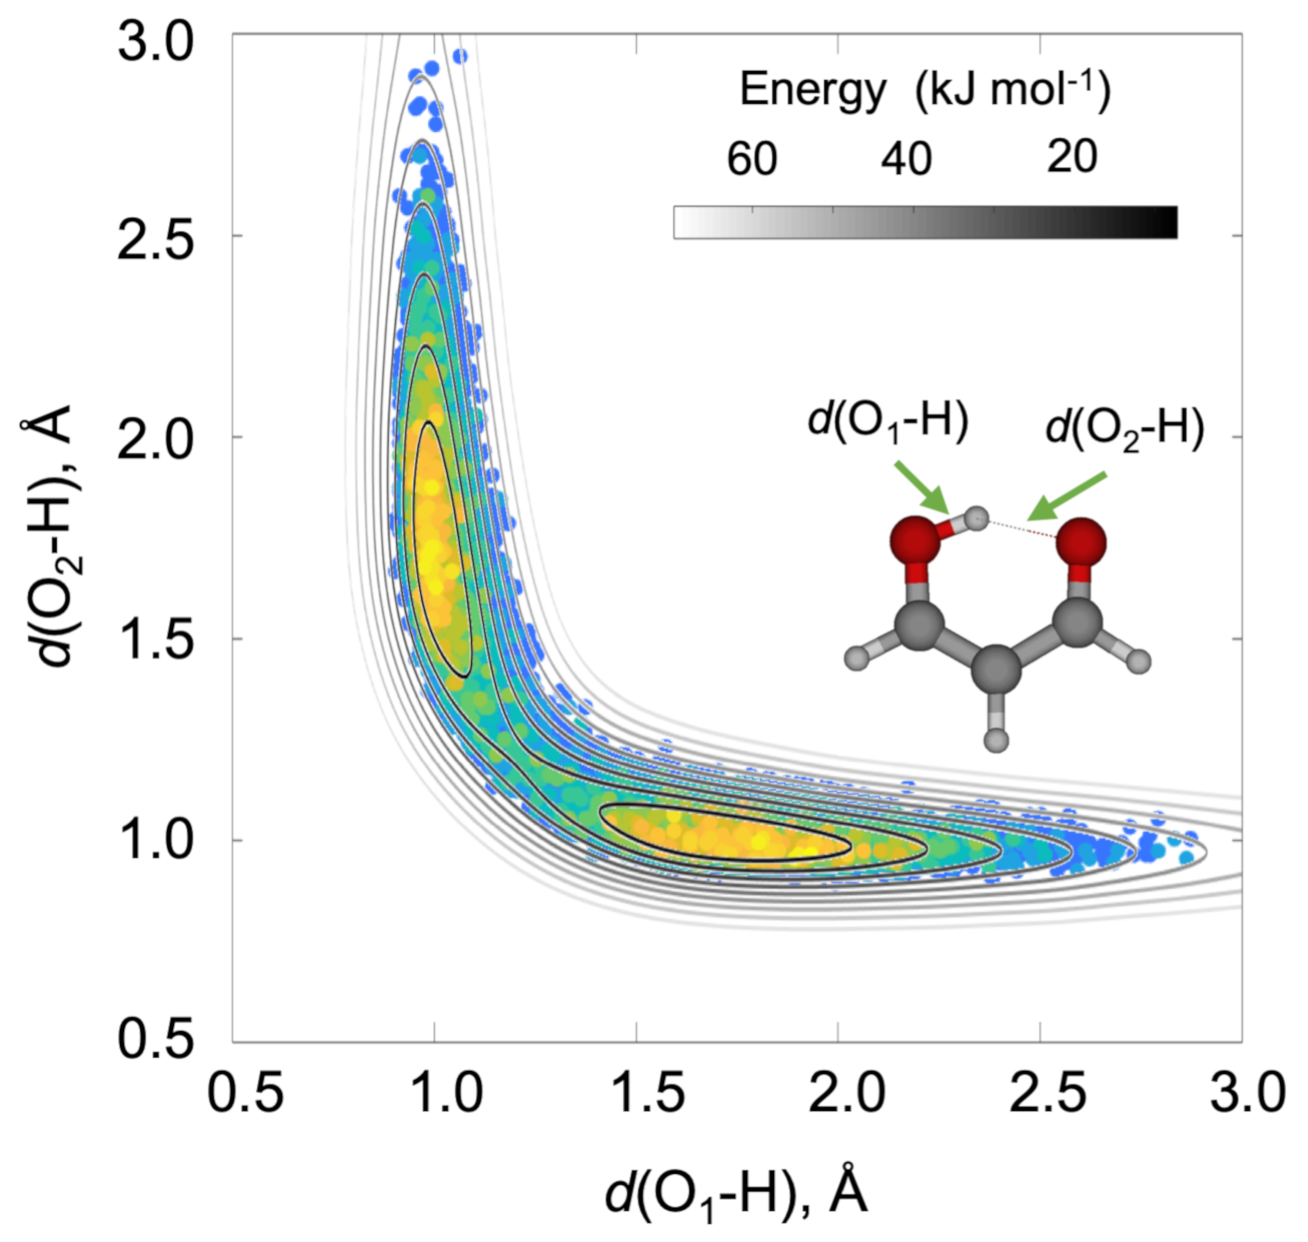
\includegraphics[width=10cm]{mtdfigure.png}
  \caption{Intra-molecular proton transfer in malonaldehyde at 298 K. Contours
    show the DFTB3-D3/3ob free energy surface of malonaldehyde obtained using
    well-tempered meta-dynamics, with collective variables $d$(O$_{1}$-H) and
    $d$(O$_{2}$-H). Each point is colored according to its sampling frequency
    during the meta-dynamics simulation, hotter colors indicating higher
    frequency.  The DFTB3-D/3ob free energy surface yields a proton transfer
    barrier of $13.1 \pm 0.4$\;kJ\;mol$^{-1}$}
  \label{fig:mtd}
\end{figure}

\subsection{\dftbp{} in Materials Studio}

\dftbp{} is included as a module in the commercial modeling and simulation
software package; BIOVIA Materials Studio (MS)~\cite{BIOVIA-MS}. \dftbp{} runs as
an in-process energy server; supplying energies, forces, and stresses to drive
the MS in-house simulations tools. Supported tasks include energy calculation,
geometry optimization, molecular dynamics, electron transport calculation,
mechanical properties, and parameterization. The module also supports
calculation and visualization of standard electronic properties, such as band
structure, density of states, orbitals, and so on. The \dftbp{} module
integrates closely with the data model and the Materials Studio Visualizer,
allowing the user to construct structures and start calculations quickly, with
fully-automated creation of the \dftbp{} input file.  The \dftbp{} module is
also supported in the MS MaterialsScript interface and the Materials Studio
Collection for Pipeline Pilot~\cite{BIOVIA-MSC}, allowing creation of more
complicated workflows~\cite{C7RA04120A,C6CP03987A}.

The \dftbp{} parameterization workflow in MS supports fitting of both electronic
parameters and repulsive pair potentials, using DFT calculations with the DMol3
module~\cite{Delley1,Delley2} as a reference. The \dftbp{} module includes
scripts for validation of parameters in terms of band structure, bond length,
bond angles, and so on, as well as visualization for the hamiltonian, overlap
matrix elements, and the repulsive pair potentials. The parameterization tools
allow extension of existing parameters or incremental development of a parameter
set. Parameters developed using the \dftbp{} module can, after conversion, be
used outside MS. Several default \dftbp{} parameter sets, generated using these
parameterization tools, are also included. In 2019, MS introduced a new
parameter set that includes the \ce{Li}, \ce{C}, \ce{H}, \ce{N}, \ce{O}, \ce{P},
\ce{F} elements and is aimed towards \ce{Li}-ion battery modeling.


\section{Software engineering in \dftbp{}}

This section presents a few aspects of our software development which may have
some interest beyond the \dftbp{} software package.


\subsection{Modern Fortran wrappers for MPI and ScaLAPACK functions}

Modern scientific modeling packages must be able to run on massive parallel
architectures to utilize high performance computing, often using the Message
Passing Interface (MPI) framework. While MPI offers a versatile parallelization
framework, its application interface was designed to support C and Fortran
77-like interfaces. This requires the programmer to explicitly pass arguments to the
MPI-routines which {\em should} be automatically deduced by the compiler for
languages with higher abstraction levels (C++ or Fortran 95 and newer versions).
In order to eliminate developer need to pass redundant information (and to
reduce associated programming bugs), we have developed modern Fortran wrappers
around the MPI-routines. These have been collected in the
MPIFX-library~\cite{mpifx}, which is an independent software project outside of the
\dftbp{} software suite, being licensed under the more permissive
BSD-license. It enables shorter MPI-calls by automatically deducing data types
and data sizes from the call signature. Additionally, several MPI parameters
have been made optional using their most commonly used value as default
value. For example, in order to broadcast a real array from the master process
to all other process, one would have to make the following MPI-call:
\begin{verbatim}
call mpi_bcast(array, size(array), MPI_FLOAT, 0, comm, err)
\end{verbatim}
while MPIFX-wrappers reduces it to a much shorter and less error-prone line:
\begin{verbatim}
call mpifx_bcast(comm, array)
\end{verbatim}
where \verb|comm| is an MPIFX derived type containing the MPI-communicator. The
type (\verb|MPI_FLOAT|) and number of broadcasted items (\verb|size(array)|) are
automatically deduced. The process initiating the broadcasting has been assumed
to be process 0 (master process) as this is probably the most common use case,
but can be customized when needed with an optional parameter. The error
argument is optional as well, if it is not passed (as in the example above),
the routine would stop the code in case of any errors.

Likewise the commonly used parallel linear algebra library ScaLAPACK uses
Fortran 77 type interfaces. The open source SCALAPACKFX
library~\cite{scalapackfx} offers higher level modern Fortran wrappers around
routines used by \dftbp{}.


\subsection{Fortran meta-programming using Fypp}
Although the latest Fortran standard (Fortran 2018) offers many constructs to
support modern programming paradigms, it does not allow for generic template
based programming. This would avoid substantial code duplication and offer
useful meta-programming capabilities for Fortran programmers. We have developed
the Python based pre-processor, Fypp~\cite{fypp-repo}, which offers a workaround
for the missing features. Fypp is used during the build process to
turn the meta-programming constructs into standard Fortran code. The
Fypp project is independent of the \dftbp{} software package and is licensed
under the BSD-license, being also used by other scientific software packages,
for example by the CP2K code~\cite{cp2k-repo} and both the MPIFX and the
SCALAPACKFX libraries.


\section{Summary}

\dftbp{} is an atomistic quantum mechanical simulation software package allowing
fast and efficient simulations of large systems for long timescales. It
implements the DFTB- and the xTB-methods and various extensions of those, among
others range-separated functionals, multiple methods of excited state
calculations and electron transport simulations. It can be used either as a
standalone application or as a library and has been already interfaced to
several other simulation packages. \dftbp{} is a community developed open source
project under the GNU Lesser General Public License, which can be freely used,
modified and extended by everybody.

\begin{acknowledgments}
  The authors, especially B.~Hourahine and B.~Aradi, thank Gotthard Seifert for
  his suggestions and insights into Density Functional Tight Binding throughout
  the development of the \dftbp{} code. B.~Hourahine acknowledges EPSRC grant
  EP/P015719/1 for financial support. B.~Aradi and T.~Frauenheim acknowledge the
  research training group DFG-RTG 2247 (QM3). C.~Camacho acknowledges financial
  support from the Vice-rectory for research of the University of Costa Rica
  (grant 115-B9-461) and the Oak Ridge Leadership Computing Facility at Oak
  Ridge National Laboratory (ORNL), which is managed by UT-Battelle, LLC, for
  DOE under Contract No. DE-AC05-00OR22725.  S.~Irle acknowledges support from
  the U.S.\ Department of Energy, Office of Science, Office of Basic Energy
  Sciences, Chemical Sciences, Geosciences, and Biosciences Division, Geoscience
  Program.  M.~Y.~Deshaye and T.~Kowalczyk acknowledge support from a National
  Science Foundation RUI award (CHE-1664674) and a CAREER award
  (DMR-1848067). T.~Kowalczyk is a Cottrell Scholar of the Research Corporation
  for Science Advancement.  T. Dumitric\u{a} was supported by the National
  Science Foundation CMMI-1332228 grant.  R.~J.~Maurer acknowledges support via
  a UKRI Future Leaders Fellowship (MR/S016023/1). A.~M.~N.~Niklasson and
  C.~Negre acknowledge support from the U.S.\ Department of Energy Office of
  Basic Energy Sciences (FWP LANLE8AN); the U.S.\ Department of Energy through
  the Los Alamos National Laboratory; and the Exascale Computing Project
  (17-SC-20-SC), a collaborative effort of the U.S.\ Department of Energy,
  Office of Science and the National Nuclear Security
  Administration. T.~A.~Niehaus would like to thank the Laboratoire d'Excellence
  iMUST for financial support. M.~St\"{o}hr acknowledges financial support from
  the Fonds National de la Recherche, Luxembourg (AFR PhD grant CNDTEC).
  A.~Tkatchenko was supported by the European Research Council (ERC-CoG BeStMo).
  V.~W.-z.~Yu was supported by the National Science Foundation (NSF) under grant
  1450280, and a fellowship from the Molecular Sciences Software Institute under
  NSF grant 1547580.
\end{acknowledgments}

\raggedright
% Workaround to get rid of meaningless warning BibTex jnrlst
\bibliographystyle{apsrev4-1}
\bibliography{titles,references}

\end{document}
%
% ****** End of file aiptemplate.tex ******
